% Modified by Alessio Guglielmi, 1 October 2023
% Modified by Christina Keating, 4 July 2025

\documentclass[12pt,a4paper]{report}
% This document template assumes you will use pdflatex.  If you are using
% latex and dvipdfmx to translate to pdf, insert dvipdfmx into the options.

\usepackage{array}
\usepackage{Bath-CS-Dissertation}

\title{\bf Human Inspired Genetic Algorithms for Multi-Agent Evacuation Routing}
\author{Laura Powell}
\date{MSc in Artificial Intelligence\\ 
                                 % E.g.: Bachelor of Science in Computer Science
                                 %       Master of Science in Data Science
      The University of Bath\\
      2026}
\renewcommand{\bibname}{References}
%%%%%%%%%%%%%%%%%%%%%%%%%%%%%%%%%%%%%%%%%%%%%%%%%%%%%%%%%%%%%%%%%%%%%%%%%%%%%%%%
%%%%%%%%%%%%%%%%%%%%%%%%%%%%%%%%%%%%%%%%%%%%%%%%%%%%%%%%%%%%%%%%%%%%%%%%%%%%%%%%
%%%%%%%%%%%%%%%%%%%%%%%%%%%%%%%%%%%%%%%%%%%%%%%%%%%%%%%%%%%%%%%%%%%%%%%%%%%%%%%%
\begin{document}

\hypersetup{pageanchor=false}

% Set this to the language you want to use in your code listings (if any)
\lstset{language=Java,breaklines,breakatwhitespace,basicstyle=\small}

\setcounter{page}{0}
\pagenumbering{roman}

\maketitle
\newpage
%
%% Set this to the number of years consultation prohibition, or 0 if no limit
%\consultation{0}
%\newpage

\declaration{Human Inspired Genetic Algorithms for Multi-Agent Evacuation Routing}{Laura Powell}
\newpage

\hypersetup{pageanchor=true}

\abstract
$\langle$The abstract should appear here. An abstract is a short paragraph describing the aims of the project, what was achieved and what contributions it has made.$\rangle$
\newpage

\tableofcontents
\newpage

\listoffigures
\newpage

\listoftables
\newpage

%%%%%%%%%%%%%%%%%%%%%%%%%%%%%%%%%%%%%%%%%%%%%%%%%%%%%%%%%%%%%%%%%%%%%%%%%%%%%%%%
%%%%%%%%%%%%%%%%%%%%%%%%%%%%%%%%%%%%%%%%%%%%%%%%%%%%%%%%%%%%%%%%%%%%%%%%%%%%%%%%
\chapter*{Acknowledgements}

Add any acknowledgements here.

\newpage

\chapter*{}
This research has been conducted in line with the University of Bath’s ethics policy and ethical approval has been obtained through Ethics@bath: $\langle$insert ethics@bath project ID here, separate by commas if you have made more than one ethics submission$\rangle$

\newpage
\setcounter{page}{1}
\pagenumbering{arabic}

%%%%%%%%%%%%%%%%%%%%%%%%%%%%%%%%%%%%%%%%%%%%%%%%%%%%%%%%%%%%%%%%%%%%%%%%%%%%%%%%
%%%%%%%%%%%%%%%%%%%%%%%%%%%%%%%%%%%%%%%%%%%%%%%%%%%%%%%%%%%%%%%%%%%%%%%%%%%%%%%%
\chapter{Introduction}

\section{Background}

%-------------------------------------------------------------------------------
\subsection{Evacuation Routing Overview}
Evacuation routing is vital to ensure that people can efficiently and carefully get to safe locations in emergency situations. It involves routing people from dangerous areas with high levels of threat to areas of safety. The frequency of disaster has been increasing in recent decades \citep{ALDAHLAWI_2024,RITCHIE_2024} and alongside the increase in population size \citep{ALSNIH_2004} there is a larger demand for effective evacuation planning \citep{CHEN_C_2023,KAMYABNIYA_2024}. Some examples of recent disasters which include: 156 deaths in the Halloween stampede in Seoul in 2022 \citep{SON_HALLOWEEN_2025}, 2431 deaths during the Mecca Pilgrimage in 2015 \citep{GANJEH_MECCA_2016} and Cyclone Ditwah in Sri Lanka in 2025, which affected over 1.4 million people, killing 410 people \citep{WHO_CYCLONE_2026}. This rise in need for evacuation routing has resulted in new methods to improve evacuation efficiency such as controlling traffic, staging the evacuation process and providing route guidance \citep{ABBELGAWAD_2009}.

Evacuations can occur in a wide range of environments which each present different structural and behavioural challenges. Building evacuations such as offices \citep{RONCHI_OFFICES_2013}, hospitals \citep{SAHEBI_HOSPITALS_2021} and shopping centres \citep{ALBIS_SHOPPING_CENTERS_2015} involve confined spaces with limited exits and high occupant densities. Large public venues such as stadiums \citep{KUO_STADIUMS_2025}, arenas and religious locations \citep{TOPRAKLI_RELIGION_2024} involve occupants having to navigate shared corridors and exits. Then urban evacuations \citep{SARMA_URBAN_2022,ALDAHLAWI_2024} triggered by more natural events such as fires, flooding or terror incidents involve more complex networks with more options, agent unfamiliarity and large populations.

\subsubsection{Cost of uncoordinated behaviour}
Human behaviour changes in evacuation situations and can result in less effective decision-making. A key driver of these behaviours is panic, which influences individual behaviours and can spread rapidly through crowds \citep{LE_BON_2024_PANIC}. One way panic can manifest in evacuation situations is herding behaviour where people group together or towards familiar exits which can result in dangerous overcrowding and potential stampedes \citep{LUGERING_2023_STAMPEDE} increasing the risk of injury and overall clearance time. Suboptimal decision making from time pressure and incomplete information can also contribute towards this \citep{LUGERING_2023_STAMPEDE}.  As panic increases throughout the crowds these behaviours accumulate and result in dysfunctional and selfish behaviour \citep{DE_IULISIS_2023_SELFISH} often to the detriment of the evacuation population as a whole. However, in evacuations situations people can feel a sense of social belonging which resulting in altruistic and cooperative behaviour \citep{COCKING_2009_SELFISH}, which can reduce the risk of these dangerous behaviours. Given the physical dangers combined with complex human behaviours under stress, evacuation planning approaches need to account for the full range of potential human responses rather than just assuming rational actions \citep{KYRIAKIDIS_2021_CONSIDER}.

\subsection{Existing Approaches}
Evacuation planning is both a practical and legal requirement in many situations, as a result there are a wide range of existing tools and software’s used to model outcomes and create appropriate safety measures. Research by \cite{SENANAYAKE_2024_PLATFORMS} found that NetLogo, AnyLogic and Pathfinder are some of the most widely used platforms to multi-agent behaviours with NetLogo and AnyLogic being referenced in 13.8\% and 7.5\% of papers respectively. Despite the capabilities of tools like above, the broader evacuation planning literature reveals a gap between the complexity of real human behaviour and the assumptions made in practice \citep{KYRIAKIDIS_2021_CONSIDER}. \cite{LOVREGLIO_2019_SURVEY} ran an online survey of user or pedestrian evacuation models across 41 countries and found 73 different models are in use, showing there is no shared standard for evacuation modellling. In addition, they found behavioural realism what not a consideration in models selected. \cite{ALDAHLAWI_2024} performaed a systematic review of 100 peer reviewed papers on large scale evacuation planning looking at how human behaviour is modelled and how routes are optimised. They found that agent-based simulation is the dominant method for modelling showing that individual level modelling has become more of a focus, however they found that heuristics and shortest path algorithms were mainly utilised showing routing decisions are still made on shortest path assumptions.

\section{Project Aims and Objectives}

\subsection{Aims}
Considering the importance of evacuating routing, this project aims to understand the impact of modelling realistic human behaviours and environment conditions on routing performance. In particular to understand in which situations a globally optimised multi-agent routing can produce better evacuation outcomes than individually optimised greedy routing under varying human behavioural characteristics. 

\subsection{Objectives}
The objectives of this research are as follows:

\begin{description}
\item[RQ1]Implement and compare the global optimised genetic algorithm (GA) against an individually optimised greedy routing strategy across structurally different topologies and seeds to understand if network topology meaningfully affect the performance of each approach.
\item[RQ2]Evaluate the rate at which agents disperse from their origin under each routing algorithm, to understand the implications of early evacuation safety.
\item[RQ3]Determine the effect of human characteristics on evacuation outcomes by embedding behaviours into the GA fitness function. Specifically:
\begin{description}
  \item[RQ3a]Evaluate how physical limitations such as walking speed effect algorithm performance such as total evacuation time and congestion.
  \item[RQ3b]Evaluate how delayed starts effect relative algorithm performance, in particular the congestion metric.
  \item[RQ3c]Evaluate how compliance levels across the population effect the GA performance, where non-compliance agents follow a shortest path route.
  \item[RQ3d]Evaluate the impact of all human behaviours on relative algorithm performance.
\end{description}
\end{description}

\subsection{Scope}

The following is in scope for this project:
\begin{itemize}
\item Agent based evacuation simulation using abstract graph-based networks.
\item Three structurally different network topologies, aiming to reflect the different situations evacuations occur in described above.
\item Congestion modelling via node capacity constraints with simple queue-based delay.
\item Human behaviour variations in walking speed, delayed started and compliance rate.
\item Multi-seed statical evaluation across multiple random seeds per experiment.
\end{itemize}  

The following is out of scope for this project but could be a potential future extension:
\begin{itemize}
\item Real world city maps or geospatial data, instead each location in the proposed network is the same distance away from each other.
\item Dynamic Routing, instead all paths are pre-planned before the evacuation.
\item Hazard modelling, instead danger exposure is inferred from agent positions over time.
\item Additional human behaviours such as herding, panic and altruism are not considered.
\item Limited Exit familiarity, it is assumed all agents know all available exits and they have no preference to a specific exit.
\end{itemize}  

\section{Contribution to Field}
This project aims to contribute to the field in two different ways. Firstly,\cite{ALDAHLAWI_2024} research identified a gap in evacuation literature which highlighted the lack of integration of human behaviours in the routing optimisation process, such as the fitness function, instead of treating it as a analysis done retroactively. Secondly, this will provide additional information on varying compliance levels, rather than the zero and full adherence which is covered in literature. This will allow us to gain further information on when collective routing strategies break down.


%%%%%%%%%%%%%%%%%%%%%%%%%%%%%%%%%%%%%%%%%%%%%%%%%%%%%%%%%%%%%%%%%%%%%%%%%%%%%%%%
%%%%%%%%%%%%%%%%%%%%%%%%%%%%%%%%%%%%%%%%%%%%%%%%%%%%%%%%%%%%%%%%%%%%%%%%%%%%%%%%
\chapter{Literature and Technology Survey}
The following chapter will start with an overview of existing techniques utilised for evacuation modelling with additional detail on the use of genetic algorithm's for evacuation routing alongside providing additional context into the motivation for this research around human behaviours and city topology.

\section{Evacuation Modelling Approaches - REFERENCE}
Evacuation models are used to predict evacuee movement and behaviour in emergency scenarios, enabling planners to assess the effectiveness of evacuation strategies before they are needed. Early evacuation modelling treated the problem as network flow optimisation problem, routing evacuee flow as directed edges with fixed capacities (Chalmet, Francis and Saunders, 1982). This approach was operationalised into tools such as EVACNET+ (Kisko and Francis, 1985) which focused on population level metrics such as total time and bottleneck emergence, but assumed fixed traversal and no behavioural variations. Later extensions such as FPETool (Nelson, 1990) added environment dynamics such as fire and smoke, while EXIT89 (Fahy, Rita, 1991; Fahy, R, 1994) introduced pre-defined behaviour rules. However, evacuees were still not treated as individual decision makers. 

Since these early methods, the number of published articles around evacuation modelling has significantly grown (Liu et al., 2020) and research has shifted more towards agent-based modelling. Zheng, Zhong and Liu (2009) identified seven methodological approaches for crowd evacuation, including: cellular automation, lattice gas, social force, fluid dynamics, agent-based, game theory and animal-based experiments (Appendix A, Table 16). This classification helps map how evacuation modelling has moved from macroscopic flow methods towards microscopic behaviour frameworks and in particular the increase in agent-based frameworks. For this project agent-based modelling is the most applicable framework because it naturally supports explicitly representation of human behaviours that macroscopic behaviours naturally tend to aggregate away.

\section{Routing Optimisation}
\subsection{Shortest Path Approaches - REFERENCES}
The fundamental challenge in evacuation planning is determining how agents should be routed from their starting positions to safety. Shortest path techniques were first formulated by Dijkstra in 1959 (Dijkstra, 2022), whose algorithm finds the least-cost route from a starting node to all other nodes in a weighted graph. The simplest and most widely used approach is greedy routing, where each agent selects the shortest path to a known safe location (Mizumura, Taguchi and Nakamura, 2024). Greedy approaches are widely used as the default option in many evacuation planning tools as they are computationally inexpensive and require not coordination between agents (Chen, Y. et al., 2014), (Mirahadi and McCabe, 2021).

However, greedy routing assumes that all agents have full knowledge of the environment, that all exits are known and equally accessible and that individual optimality translates to collective optimality. Stepanov and Smith (2009) showed that individually optimal routing in transportation networks produced worse collective outcomes than globally coordinated routing. It has also been demonstrated that greedy routing breaks down when there are capacity constraints, congestion and time dependent conflicts (Min, Lee and Lim, 2014; Hong et al., 2018; Shahabi and Wilson, 2018), likely occuring due to locally optimal step selection.

This highlights a key limitation in shortest path approaches, although they may look efficient in isolation, they often generate congestion when many agents use them simultaneously, resulting in poor results for the population as a whole.

\subsection{Price of Anarchy - REFERENCES}
This gap between individual versus the collective optimally is defined as the Price of Anarchy (PoA)(Papadimitriou, 2001). PoA is a concept utilised in game theory (Cominetti, Dose and Scarsini, 2024) which defines the ratio between the worst case scenario and the best, thereby quantifying the inefficiency of selfish behaviour on the system (Roughgarden and Tardos, 2002; Roughgarden, 2015). Roughgarden (2003) showed that the PoA effects arises even in very small networks, meaning scalable models of city-wide evacuations can be informed by simpler examples. Fries et al. (2022) examined planned evacuation routes versus guidance from navigation systems (shortest path) and found the planned routes produces less congestion. These results reinforce that evacuation routing strategies must explicitly manage the trade-off between individual convenience and system wide efficiency.

\subsection{Metaheuristic Approaches - REFERENCES}
Metaheuristic approaches are useful for finding the balance between exploration (searching widely across the solution space) and exploitation (refining promising solutions) to tackle evacuation routing problems (Abdel-Basset, Abdel-Fatah and Sangaiah, 2018), however they do not guarentee an optimal result.

Metaheuristics are useful in evacuation routing applications as they can incorporate changing conditions and multiple objectives such as travel time and route capacity. Li, C. et al. (2025) combined a flood hazard rating with distance in Ant Colony Optimisation (ACO) and Particle Swarm Optimisation (PSO) to identify efficiency evacuation routes which avoided high risk flood areas. The improved ACO and PCO improved safety and speed respectively for the York flooding scenario. Yang, G. and Chen (2024) showed the combining simulated annealing with genetic algorithms found short and safe routes in crowded underground public spaces. Pratap and Aziz (2025) applied an ensemble of metaheuristics and found it produced more robust routes across a range of test networks with varying uncertainty levels, than simpler methods. These examples show that metaheuristics can encode richer objectives and environmental constraints but most research still treats human behaviours as external parameters rather than as an optimisation variable.

\section{Genetic Algorithms}
\subsection{Genetic Algorithm Concepts}
Genetic algorithms (GA) are a population based evolutionary metaheuristic that has been widely used in search and optimisation problems, including evacuation routing. They draw inspiration from biological evolution, using operators such as selection, crossover and mutation to evolve potential solutions over successive generations. In the context of evacuation routing, the populations typically encode a set of potential routes or collection of routes.

Each generation proceeds through the following steps and repeats itself until a termination criteria has been met. Parent solutions are selected from the population based on their fitness value using techniques such as roulette or tournament selection. Children are then generated from parent pairs through crossover operators such as single or multi-point, before being potentially modified through mutation to maintain diversity and prevent premature convergence. After the children are generated, they are evaluated and a new population is selected for the next generation. The fitness function can incorporate multiple objectives and constraints, to assess the quality of each route configuration. A known limitation is the high computational cost of evaluating complex fitness functions, especially in high dimensional evacuation networks.

\subsection{Use in Evacuation Routing - REFERENCES}
von Schantz and Ehtamo (2022) combined a genetic algorithm with a social force model to identify the best locations to place rescue guides in emergency situations in a fictional building whilst also minimising congestion effects and total evacuation time. Saadatseresht, Mansourian and Taleai (2009) incorporated distance from a safe area, exposure to risk and total time into their objective function to identify potential evacuation plants. Cotta and Gallardo (2024) optimised placement of exits and incorporated factors such as last evacuee time and average time, to create a score for each potential exit layout. They found the evolutionary algorithm consistently found better layouts.

Despite these advances in research, human behaviour is often oversimplied or not explicitly modelled. Research which has explicity modelled human behaviour include: Hansen et al. (2016) by rewarding plans which kept evacuees together (herding) and Dembytskyi and Dorogyy (2017) who utilised GAs to optimise a neural network to better model the state of people in crowds including route decisions and risk tasking. These studies show that GAs can be used both for route optimisation and for approximating human behaviour but there remains a gap in literature regarding how to embed human behaviour rules directly into the GA routing process.

For this project, GAs have been chosen because they are population based (providing multiple routing policies), multi-objective compatible and well suited for encoding evacuation routes over complex networks.

\section{Human Behaviour in Evacuations}
\subsection{Importance of Human Behaviour in Modelling - REFERENCES}
Behaviours such as panic, conformity and familiarity shape evacuation (Kuligowski and Gwynne, 2010; Caunhye, Nie and Pokharel, 2012; Zhou et al., 2019). When models neglect these behaviours estimated routes, safety levels and evacuation times can be underestimated, leading to overly optimistic planning assumptions (Keykhaei et al., 2023; Giardini et al., 2024).

Hofinger, Zinke and Künzer (2014) identified key factors which can influence evacuations, including physical limitations (mobility, age, disability), cognitive aspects (risk perception, attention, familiarity), motivational factors (anxiety, trust) and social influences (group attachment, following others). They argue that current evacuation simulations often oversimplify these by assuming “uniform, highly rational evacuees” and call for better data and validated variables for human behaviours in evacuations. Templeton et al. (2024) review of agent-based modelling papers showed most modern simulations don't consider human behaviour and those which do are often simplistic and not grounding in theory. This motivates the need for empirically informed representation of human behaviour that are tightly integrated with evacuation routing and optimisation, rather than added on after the fact.

\subsection{Existing research on the impact of human behaviour - REFERENCES}
Wang, J. et al. (2025) used Pathfinder to model pedestrian flow in 3D environments and found controlling or reducing flow improved evacuation efficiency by 15\%, but in severe panic scenarios evacuation efficiency decreased by 16\%, highlighting that states such as panic can negatively impact routing strategies. Li, Jianxun et al. (2024) embedded characteristics such as age and altruism probability into a social-force evacuation model. They found increasing the help probability from 10\% to 40\% improved total evacuation time but after this point there was no additional improvement, suggesting some positive social behaviour can improve total time. Moussaid et al. (2016) used a virtual environment platform with human participants to study how participants moved under different high stress evacuation conditions. They found that herd behaviour naturally arose and resulted in congestion at exit points and bottlenecks even when other routes or exits were less crowded. This implies real evacuees do not just pick the shortest path but instead react to other evacuees’ movements which may not be fully captured in shortest path approaches. Wang, Y., Kyriakidis and Dang (2021) reviewed evacuation modelling over time from both pedestrian and vehicle evacuations. They examined different human behaviours such as pre-movement delay and social influence, and compared them to how models represented evacuees. They found that research which only models the route choice of evacuees can result in missing vital decisions, such as when to leave and who to follow, which impact later decisions and outcomes.

Şahin, Rokne and Alhajj (2019) highlighted the importance of modelling people as decision making agents including factors such as speed, size, familiarity and importantly decision-making rules. Comparing the results to simpler models, such as shortest path, showed exit time and usage differed significantly. They highlighted several next steps around grounding human behaviour in real data, richer cognitive architectures, dynamic environmental models and incorporating it into frameworks to design and test evacuation policies. Collectively, these studies how that small changes in behavioural assumptions can have large, non-linear effects on evacuation time and safety.

\subsection{Research Gaps and Opportunities}
Aldahlawi, Akbari and Lawson (2024) systematic review of 100 papers identified that although there is research in Agent Based Simulations being used to model behaviours, optimisation driven techniques such as heuristics and traffic assignment still dominate evacuation route planning. The integration between decisions and route choices is underutilised in optimisation approaches and required further research. They also highlight there is an absence of literature exploring different contexts such as university campuses and the differing facilities, vehicle evacuations and signage systems, industrial cities and country-sides with varying familiarity and environmental risk (e.g. increased fire spreading). This motivates the need for frameworks that embed empirically informed human‑behavioural rules into evacuation optimisation across different settings, (e.g., campuses, mixed‑traffic environments, and heterogeneous populations).

In particular, prior GA evacuation work has largely focused on route length, risk and infrastructure layout but has not typically evolved the human behaviours as part of the genetic search process. This project aims to bridge this gap by designing a genetic algorithm-based framework that considers human behaviours as part of the optimisation process across different network topology settings.

\section{Network Topology and City Structures - REFERENCES}
Evacuations occur in a range of different scenarios; evacuation planning needs to be tailored to each of these contexts because different physical and social factors will dominate. In buildings, evacuation outcomes depend heavily on the capacity of corridors and stairs, visibility and familiarity of occupants with the layout (Fu et al., 2024). In city-scale environments, dense populations require considerations of exit placement, medical services, management of traffic flow patterns and agent behaviour, for example do all agents become aware of the evacuation at the same time or do they become aware in stages (León et al., 2019; Borowska-Stefańska et al., 2025). All these factors and city structures strongly shape where bottlenecks and congestion develop which in turn influences evacuation time and safety. By better understanding how agents flow through different networks, there is a better understanding of how to create routing policies and plans which adapt to human behavioural patterns rather than assuming uniform shortest path behaviour. This project uses multiple network topologies as environments to simulate the multi-agent algorithm and to evaluate how behaviourally informed routing affects evacuation performance.

%%%%%%%%%%%%%%%%%%%%%%%%%%%%%%%%%%%%%%%%%%%%%%%%%%%%%%%%%%%%%%%%%%%%%%%%%%%%%%%%

\chapter{Design}

\section{Research Aims and Design Scope}
This project aims to utilise genetic algorithms with human behaviours incorporated into the fitness function to better understand the impact of human behaviours on key evacuation metrics. This will be compared against a shortest path algorithm across the following human behaviours: delayed starts, compliance and physical limitations (represented through walking speed). These different behaviours will be evaluated across three fictional network topologies: grid-like, moderate-complexity and bottleneck-constrained areas. 

The following section breaks down the design decisions for the key components of the simulation framework in this project. The project is structured as an agent-based simulation where:
\begin{itemize}
\item Agents represent evacuees with distinct behavioural states and movement constraints.
\item The environment is a graph-based network, instantiated in three different topologies.
\item Two routing algorithms are compared: a greedy shortest path baseline and a genetic behaviour aware algorithm.
\item The experiment pipeline runs multiple simulations across a range of seeds and records the evacuation metrics for comparison.
\end{itemize}

\autoref{fig:architecture-design} provides an architecture diagram that illustrates the overall framework, showing the interactions between the environment, agents, routing algorithms and experiment evaluation.

\begin{figure}[h]
    \centering
    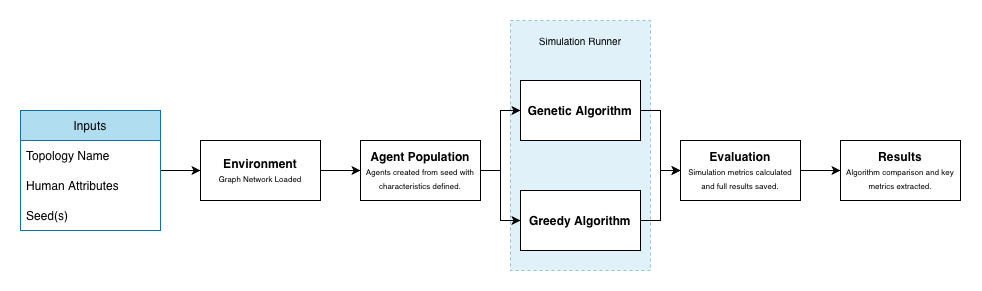
\includegraphics[width=0.8\textwidth]{dissertation_images/architecture_diagram_design.png}
    \caption[Architecture Diagram]{Architecture diagram showing the  project framework connecting the input parameters through environment, agent creation, routing algorithms and evaluation.}
    \label{fig:architecture-design}
\end{figure}

\section{Design Framework}
\subsection{Environments}
Three network topologies were picked in order to represent the different conditions which evacuations can occur. They are represented as abstract graphs rather than spatial or geospatial maps, with nodes corresponding to intersections and edges corresponding to roads or corridors. Representing the topologies as spatial or geospatial graphs would have been more realistic, capturing factors such as one-way streets, distances and elevation which all impact evacuation routing and would also be immediately applicable to real locations. However, by using simplified examples of cities we can guarantee a comparable performance and ensure that the difference between the algorithms is due to the routing strategy and human behaviours rather than the network layout. Fictional topologies also allow for the networks to constructed to deliberately represent different conditions.
For all the topologies the number of start and exit locations will be held constant in order to focus on the network structure rather than confounding the results with number of exits (more could cause faster evacuations) or start locations (less could lead to more congestion at the beginning). This assumption is idealised as in real evacuations the number of exits and starts will varying widely, such as high-rise buildings, stadiums or city evacuations, so we could be underrepresenting the number of safe locations which influences many evacuation outcomes.

Additionally, for the following topologies the edge weight is set to one in order to simplify the model and focus on the structural properties of the network. This assumption treats all edges with having equal travel costs which avoids the need to specify distances. For the same reason, all nodes have the same capacity constraints, assuming every agent location can hold the same number of evacuees. If this capacity is exceeded, congestion forms at the node blocking further movements until the density decreases. When the nodes reach capacity, this will be representing the real-world bottlenecks which appear in evacuations such as in corridors or narrow streets. This simplification has limitations as in real world evacuations, routes differ in length and agent locations have differing capacities. Ignoring these variations can mask important routing effects such as avoiding hazard areas or longer distance routes.

The above design choices have been selected as this is an initial exploratory study of network topology and human behaviours and allow for a cleaner comparison of routing behaviour and human behaviours across the network structures, but it does limit the comparison of the results with empirically informed networks.

The first grid like topology represents a grid city, such as a city from in a dense urban area. The edges between nodes represent the streets between blocks of buildings and agents are not permitted to move “into buildings”, so all movement is constrained to the street network.  The high connectivity and multiple parallel routes will create a wide range of paths to exits. This makes the grid topology a useful test case for studying how agents distribute themselves across many alternative routes.

The next is the moderate-complexity topology, this represents a partially obstructed evacuation environment, such as a scenario where certain routes have become blocked or inaccessible. By removing a subset of nodes and edges from the grid the networks will product uneven route distribution where some edges become heavily dependent in reaching an exit location and short alternative routes may not always be an option. This makes the moderate topology useful for comparing the routing strategies when paths become more constrained but there are still alternative paths.

The final topology is bottleneck-constrained, this is meant to represent evacuation scenarios where there are limited initial path choices. An example of this might be stadium or venue evacuations, initially all evacuees must follow limited routes but once out the initial area they have more options to finding safe locations. By limiting the number of initial edges from the start nodes, agents will have to share these initial routes resulting in high congestion levels. This makes the bottleneck-constrained topology a useful test for understanding how routing strategies perform when the environment created unavoidable conflicts.

\subsection{Agents}
Agents will have a range of individual characteristics representing walking speed (physical limitation such as age and vulnerabilities), delayed starts (not all agents will react to situations at the same rate) and a compliance (will agents follow indicated routes or focus on selfish routes to get to safety). The agents’ characteristics and start location in each topology will be the same across experiment seeds and will be randomly generated at the start of the simulation. This will ensure that the comparison between the routing algorithms will be due to routing choices and not the variation is not due to start locations or different behaviours (e.g. one algorithm has a quicker average walking speed). For all the following attributes, the model assumes they remain constant over time. This simplification improved reproducibility and analysis of the outcomes, however it is not reflective of real evacuation situations, where agents will experience dynamic changes such as increasing panic levels or shifting compliance.

The agents walking speed will be encoded as three different options: one, two or three. These categories represent the time it takes to traverse an edge with speed one the quickest someone could walk. This simulation assumes walking speed is not interrupted by terrain or environmental factors. A standard walking speed used in most research is 1.35m/s identified by Fruin (1970), studies have shown this can increase to 1.6-2.2m/s (Zhao et al., 2017) in evacuation situations. Additionally, GOV UK (2025) highlighted that people with limited physical abilities walk in the range of 0.2-0.5m/s. The three walking speeds selected represent these speeds in a simpler way, where slowest speed (0.5m/s) represents approximately a third of the speed of the fastest walkers (1.6m/s). These discrete walking speeds are a simplification than a more realistic continuous distribution so it may not capture full human variability found in evacuations. Each agent is randomly assigned one of these categories according to proportion of the population that these groups represent in the evacuation scenario, for this project these where set as 60:30:10\% respectively. This weighting assumption allows the model to capture the impact of different weights on evacuation time and congestion, but this is a significant simplification of reality as the mix of abilities will vary by building type, for example universities are likely to have more abled bodied people than a hospital.

Agents will also be encoded with differing delayed start values; zero, one or two. In evacuation situations it is rare that everyone begins moving at exactly the same time, and even when people become aware simultaneously, they do not all react or evacuate at the same pace. This delayed start attribute represents the differing pre-movement delays which are commonly observed across human evacuations (Fahy, R.F. and Proulx, 2001). In this experiment the delay values represent the number of time steps an agent will wait before starting the exit route journey: zero represents an immediate response, one a moderate delay and two the longer delayed start such as waiting for an explicit evacuation instruction. Forssberg et al. (2019) analysed 2486 data points and found that pre-movement times can be represented as a lognormal or loglogistic distribution, so the three delay levels will be assigned to agents following a discrete approximation of this with [0.4, 0.4, 0.2] respectively. Although this is simplification of the continuous variation in real pre-movement, and assumes all people will delay, it captures the general right skewed nature of evacuation start behaviour. Additionally, this model assumes delay is fixed to the start of the journey, although delays can occur at any point as information’s spreads or risk becomes clearer (Bode and Codling, 2018). 

The final human attribute which will be evaluated is a human compliance attribute. For this each agent will be assigned a Boolean value to indicate if they can be part of the genetic algorithm route optimisation (1 = compliant) or if they instead will choose the selfish, shortest path (0 = non-compliant). This will directly encode a common trade off in evacuation behaviour between following centralised guidance and pursuing individually optimal routes. Encoding compliance as a single binary value, simplifies complex human behaviours as agents may choose to be compliant in some sections of an evacuation process, for example near authority figures but not otherwise. However, it allows for an analysis of how the overall evacuation outcomes vary as compliance becomes more of a risk.

The design of this project focuses on walking speed, delayed starts and routing compliance because they directly affect evacuations time, congestion and the gap between greedy and centrally optimised routing. Other attributes which are present in evacuations such as panic, herd behaviour or familiarity also impact evacuation time but become more complex to model. 

\section{Routing Algorithms}
\subsection{Genetic Algorithm}
The GA will follow the traditional methodology with changes to the fitness function to ensure that human behaviours are considered as part of the optimisation process. 
The fitness function will focus on the total evacuation time for all agents across the chromosome. Each chromosome encodes a candidate solution as a list containing the proposed path for the corresponding agent. In traditional genetic algorithm terminology, a gene is a single position in the chromosome, and in this implementation each gene is a single agent’s path. At the initialisation phase of each chromosome a random path is created from a pre-defined start point to any exit in the network. In order to ensure that each chromosome has a reproducible, random path a Key Manager will be utilised, this ensures the results can be reproduce and that each chromosome has a different starting path ensuring population diversity. In order to simplify the modelling process and avoid the genetic algorithm becoming stuck with long routes, each time a route is created and updated any potential loops are removed from the path, this assumes that evacuees would not just keep walking in circles, although it is worth noting that in reality this can happen especially in scenarios where people are panicked and not paying full attention.

An agent’s total evacuation time is made up of two key components: the length of the path (how many nodes from start to exit points) and the amount of congestion experienced. An agent will experience a congestion delay if they are at a node which the capacity is exceeded, and they are not selected as a node to move through the node. The agent will wait at the node until the number of agents drops below the capacity or they are selected as a node to go through. Any agent which was previously at the node will have a priority over new agents arriving at the node for the first time steps they arrive at but after that agents are randomly selected as to whether they progress or have to wait. Another option considered was a weakly time dependent model for congestion where delays didn’t propagate forward, however this would greatly exaggerate the congestion effect where agents are consistently getting stuck at the same nodes each time step. 

Additionally, when walking speed and delayed start behaviour are turned on, they will affect fitness function. The agents walking speed will become a multiple to the path length so slower agents will take three timesteps to traverse between nodes and delayed starts will stop agents from moving for the initial delay period, adding a delay to the total time. The compliance behaviour will not directly influence the fitness function but instead replaces the GA path with the shortest path. The fitness function will likely take the maximum agent path value, however values such as mean and median will be considered to ensure the GA balances overall vs worse performance. While this fitness function explicitly optimises paths in the presence of human behaviours, it treats each agent’s path as fixed once generated and cannot adapt to dynamic changes during a simulation which limits its ability to represent changing risks in real time.

\begin{equation}
    f(c) = \max_{i \in \mathcal{A}} (S_i \cdot \mathrm{length}(p_i) + D_i + C_i)
    \label{eq:fitness-function}
\end{equation}

\noindent The fitness function $f$ for a chromosome $c$ seen in \autoref{eq:fitness-function} is made up of: $\mathcal{A}$ is the set of agents and for each agent $i$ the walking speed ($S_i$), $length$ of the path ($p_i$), delayed start ($D_i$) and congestion delay ($C_i$). For delayed starts and walking speed if they are not turned on for an experiment they are set to the default values, 0 and 1 respectively.

The performance of the GA depends on the implementation and tuning of its core operators: parent selection, crossover, mutation and survivor selection.

The genetic algorithm will use a roulette parent selection operator. Roulette select involves taking the population of chromosomes, ordering them by their fitness value and assigning each a probability of being selected as a parent in the next evolution proportional to its fitness value. This method ensures that better solutions have a higher chance of moving through the generations whilst still ensuring that lower fitness solutions still can come through in order to maintain diversity. One concern with roulette selection is that if a chromosome dominates the wheel of finesses, it could cause premature convergence. To monitor this the metrics in \autoref{table:parent-selection} will be used during experimentation. If any show undesirable behaviours, the algorithm may switch to an alternative selection method such tournament or rank selection will be used.

\begin{table}[htb]
  \bigskip
  \begin{center}
    \begin{tabular}{| p{2.5cm} | p{5.2cm} | l | p{5cm} |}
      \hline
      Metric & Reason & Equation & Thresholds \\
      \hline
      \hline
      Coefficient of Variance & How spread out the fitness values ($f$) are in comparison to the mean value. & $\frac{std(f)}{mean(f)}$ & $\leq 5\%$ values are too similar and $\geq 30\%$ one solution is dominating. \\

      Dominance Ratio & Shows the ratio of best to worst fitness values. ($f$) & $\frac{\max(f)}{\min(f)}$ & $<1.5$ results are too similar and $>10$ the best solution dominates. \\

      Best Wheel Share & Proportion of the wheel the best chromosome takes up. & $\frac{\max(\mathrm{inverse\ f})}{sum(\mathrm{inverse\ f})}$ & Between $20-40\%$. \\

      \hline
    \end{tabular}
  \end{center}
\caption{Parent selection performance metrics}
\label{table:parent-selection}
\end{table}

In the crossover operator, for each set of parents the algorithm will first check whether child candidates will be created according to a pre-defined crossover probability. If crossover occurs, the two parent chromosomes are taken and the algorithm loop through each agent. For every agent we check to see if the paths have an overlapping crossover point, if they don’t then the parent paths are carried directly forward into mutation. If they do a random overlap point is selected and the paths for the agents are swapped, because crossover is performed at the agent‑level and only uses overlapping nodes as crossover points, the resulting paths remain valid, and there is no need to add extra logic to “repair” invalid routes or to fall back to greedy shortcuts. This simplifies the comparison between routed paths and ensures that the GA‑search space remains constrained to feasible evacuation routes. However, agent level crossover can limit the space of possible new ideas as the algorithm might struggle to combine ideas from different routing patterns which could slow exploration.

For the mutation operator, for each agent in a chromosome is tested independently against the mutation probability threshold. In this implementation, mutation occurs by allowing an agent to select a new exit to go to (including their current one), then a point along the agent’s path is selected and a new path is creating using an epsilon-greedy path selection. This method was selected over a purely greedy path selection strategy as it preserves a balance exploration vs exploitation. This technique keeps routes valid; however, it still likely oversimplifies human behaviour changes in evacuation as it assumes local path adjustment rather than a broader change in decision making. It also does not explicitly model panic-driven behaviours or communication effects, instead representing these indirectly through the balance between exploration and exploitation

The final operator in the GA is the survivor selector operator, in most literature the next generation of the population is made up of the highest fitness between children and parents (elitism). For this project a hybrid percentage-based selection approach has been selected where only a certain percentage of the parent selection will be carried through to the next generation. This method was selected in order to preserve exploration by avoiding discarding immature route structures before they have the chance to evolve. This approach may result in a delayed convergence in comparison to a pure elitism approach as weaker parents can survive for longer than necessary. To validate this choice three variants of survivor selection will be compared to ensure the algorithm converges: hybrid percentage, elitism and children only.

The termination strategy for the genetic algorithm will be when it reaches a defined maximum number of generations. This straightforward approach ensures computational traceability while allowing sufficient time for convergence. This parameter will be tuned experimentally to balance solution quality against runtime. However, this approach still risks stopping before convergence or unnecessary computation.

The genetic algorithm will have a significant number of parameters which will need tuning before the results can be ran and analysed, \autoref{table:ga-parameters}. Due to the high computation costs of full grid search across multiple parameters and scenarios, a sequential tuning approach is used instead. Each parameter will be optimised across multiple seeds in the moderate topology, while hold other fixed at those widely used in literature or the tuned value. The moderate topology has been used as it should capture the key congestion dynamics affecting evacuation time without extreme edge cases. The key limitation of this approach is that it assumes parameters independence and could miss important interactions and result in suboptimal performance across other topologies.

\begin{table}[htb]
  \bigskip
  \begin{center}
    \begin{tabular}{| p{3cm} | p{6.5cm} | p{5cm} |}
      \hline
      Parameter & Description & Options \\
      \hline
      \hline
      Crossover Threshold & Threshold in which if less than crossover will occur. & [0.4, 0.5, \textbf{0.6, 0.7, 0.8}, 0.9]\\

      Mutation Threshold &  Threshold in which if less than mutation will occur. & [\textbf{0.01, 0.05}, 0.1, 0.2, 0.3, 0.4] \\

      Epsilon & Threshold to decide in an agent should pick a random or greedy node. & [\textbf{0, 0.2}, 0.4, 0.6, 0.8, 1] \\

      Maximum Evolutions & Number of evolutions before the algorithm is terminated. & Maximum 200 and metrics analysed across evolutions. \\

      Population Size & Size of population used. & [5, 10, 20, \textbf{50, 100}, 200]\\

      Number of Agents & Number of agents in the simulation. & [10, 20, 50, 100, 200] \\

      Fitness Function ($\alpha$) & Fitness function aggregation formula for each chromosome. & Max, mean and median and $(\alpha * \max - (1-\alpha)*median)$ for $\alpha \in [0.35, 0.5, 0.8]$. \\

      Parent Selection Method & Approach to parent selection. & Elite Percentage, Elite, Children only \\

      Survivor Selection Method & Approach to decide what the next population will be. & Roulette, Tournament (N=3), Tournament (N=5) \\

      \hline
    \end{tabular}
  \end{center}
  \caption[Genetic Algorithm parameters]{Genetic Algorithm parameters, bold highlights are ones which are widely used.}
  \label{table:ga-parameters}
\end{table}

\subsection{Shortest Path Baseline}
For the shortest path baseline, a greedy algorithm will be used to route each agent independently to find the shortest path to any exit from their pre-defined starting node. In the situation where there are multiple shortest paths to different exits, or to the same exit, a random path from the options will be selected. This choice to select from all possible routes, rather than the first found route in the algorithm, reflects real evacuations where evacuees will naturally split across equivalent exits, for example, if there were two stairways out of a stadium for example the population would likely split across the two equally. First-found selection would be unrealistic from the increase in artificial congestion levels from all agents taking the exact same route. Greedy shortest path is the industry standard in evacuation simulation software. So, picking another metaheuristic baseline would test metaheuristic vs metaheuristic rather than the impact of behaviour on the estimates used for evacuation planning.

\section{Experimental Design}
The parameters found in \autoref{table:ga-parameters} will be tuned and selected ahead of the following experiments. The experiments will be done across all three topologies and 10 different seeds to validate the statistical significance.

The first experiment will compare the performance of the greedy algorithm vs the genetic algorithm with no human behaviours just comparing congestion, dispersion and total evacuation time, directly addressing RQ1 and RQ2. This allows us to understand what the gap looks like before any human behaviours are added. This establishes the baseline performance gap due to selfish and global optimisation.

The second experiment introduces agent walking speed multipliers (x1, x2, x3), addressing RQ3a testing how physical limitations affect both the algorithms performance and if the genetic algorithm adapts routes to priorities slow agents and if congestion hotspots shift dynamically.

The third experiment tests delayed starts (+0, +1, +2) to address RQ3b, to examine how temporal staggering impacts congestion and total evacuation time and if the genetic algorithm learns start-time aware routing patterns.

The fourth experiment varies compliance rates, from 0\% (no compliance) to 100\% (full compliance), addressing RQ3c. This experiment will help to determine the breakdown threshold where selfish behaviour degrades the global optimisation benefits.

The fifth experiment combines all human factors (speed, delays and compliance) to address the final research question (RQ3d), this will quantify the cumulative impact of realistic behaviours on the genetic algorithm and greedy performance gap. This experiment will also be used for the dispersion analysis of agents near start zones over time (RQ2).

\section{Metrics}
\subsection{Genetic Algorithm Monitoring Metrics}
The metrics in \autoref{table:ga-monitoring-metrics}, were used to track the performance of the genetic algorithm (GA) over the evolutions.

\begin{table}[htb]
  \bigskip
  \begin{center}
    \begin{tabular}{| p{3cm} | p{5cm} | p{6.5cm} |}
      \hline
      Metric & Description & Reasoning \\
      \hline
      \hline
      Best Fitness Value & Lowest value across all chromosomes. & Tracks if the GA is finding better solutions over time. \\

      Mean Fitness Value & Average value across all chromosomes. & Indicates the overall quality of the population. \\

      Worst Fitness Value & Highest value across all chromosomes. & With the above used to understand the spread of the population. \\

      Mean Path Length & Average number of nodes across all agent paths. & Isolates if improvements are from shorter routes or reduced congestion. \\

      Mean Congestion Delay & Average congestion penalty across all agents. & Isolations congestion to see if the GA is successfully distributing agents. \\

      Population Diversity & A measure of how varied the chromosome are. & Indicates premature convergence or if stuck in local optima. \\

      Run Time & Each stage and total run time. & Understand the impact of parameter choices versus performance. \\

      \hline
    \end{tabular}
  \end{center}
\caption{Genetic Algorithm monitoring metrics per evolution}
\label{table:ga-monitoring-metrics}
\end{table}

\subsection{Evaluation Metrics}
The metrics in \autoref{table:experiment-metrics} will be calculated and compared across multiple seeds to assess algorithm performance within each topology. In addition to the metrics listed, research question specific measures are reported in the results section where required.

\begin{table}[htb]
  \bigskip
  \begin{center}
    \begin{tabular}{| p{3.5cm} | p{5.5cm} | p{5.5cm} |}
      \hline
      Metric & Description & Reasoning \\
      \hline
      \hline
      Total Evacuation Time & How long to get all agents out (i.e.worst performing agent). & Primary metric for overall performance. \\

      Average Evacuation Time & How long on average for an agent to exit. & Helps to understand the average population. \\

      Mean Congestion Delay & How long on average were agents delayed. & Isolates if performance is drive by cognestion management. \\

      Mean Path Length & On average how long was the path the agents took (i.e. number of nodes). & Isolates the path length other factors e.g. congestion and walking speed. \\

      Route Efficiency & Comparison of the shortest path length versus the actual path length. & Captures how much path deviation was required to reduce congestion (GA only). \\

      Dispersion Rate & Number of agents remaining within a number of nodes (N) from their starting position. & Measures how quickly agents leave the initial danger zone during early evacuations. \\

      \hline
    \end{tabular}
  \end{center}
\caption[Algorithm comparison metrics]{Metrics to compare algortihm performance for the best solution.}
\label{table:experiment-metrics}
\end{table}

\section{Assumptions and Limitations}
The key assumptions have been discussed above, but a summarised version can be found below.
\begin{itemize}
  \item Agents are rational route choosers.
  \item Static Environment with no dynamic hazards.
  \item All edges have equal weight and all nodes have equal.
  \item Agents have fixed behavioural throughout a simulation.
  \item Start and exit locations are fixed across seeds so performance differences come from the routing strategy not the change in setup.
  \item Paths are loop-free to avoid unrealistic cycling.
\end{itemize}

\vspace{1em}
Additionally, a summarised version of the previously discussed limitations is:
\begin{itemize}
  \item Human behaviour is simplified into discrete categories so full variability is not captured.
  \item Behaviour does not evolve over time so simplifies human behaviours.
  \item Congestion is abstracted through node capacity rather than fine-grained interactions.
  \item Topology is fictional and idealised, allowing for comparison but limits real world applications.
  \item Edge weights and node capacities are uniform, so route length and terrain difficulty are not represented.
  \item Sequential tuning may miss parameter interactions and not transfer perfectly across topologies.
\end{itemize}

%%%%%%%%%%%%%%%%%%%%%%%%%%%%%%%%%%%%%%%%%%%%%%%%%%%%%%%%%%%%%%%%%%%%%%%%%%%%%%%%
\chapter{Implementation and Testing}
\section{Implementation Overview}

The simulation framework was implemented in Python, chosen for the wide availability of libraries such as NetworkX, NumPy and JAX. NetworkX provides the ability to construct graph networks and has unbuilt graphical functions such as shortest path functionality. NumPy and JAX were used throughout the code for numerical operators and seed generation. The code base is structured around eight core classes in \autoref{fig:code-classes}. A link to the full code base can be found in **APPENDIX ?**.

\begin{figure}[h]
    \centering
    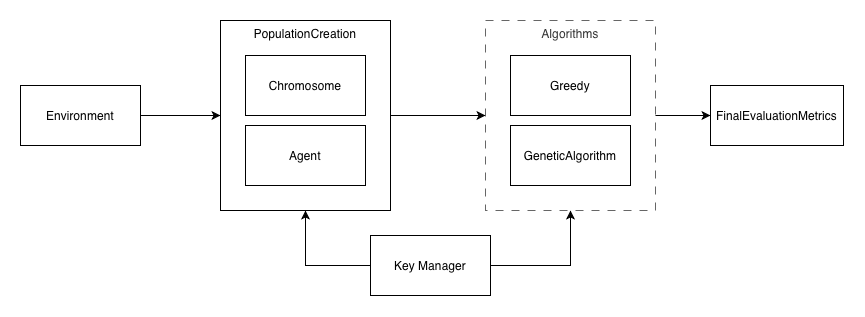
\includegraphics[width=0.8\textwidth]{dissertation_images/code_class_flow.png}
    \caption[Code Class Structure]{Code Classes and interactions in simulation creation.}
    \label{fig:code-classes}
\end{figure}

This chapter documents the key implementation decisions made during development, testing and validation prior to running the main experiments.

\section{Environment Implmentation}
Three network topologies were constructed programmatically in Python using the NetworkX library, each derived from a common base 6x9 grid graph. The start and exit locations across the three topologies did not change and only edges and nodes were removed to create the different layouts. By keeping the locations consistent it ensures the difference are from the network structure rather than number or placement of safe locations, however this is a simplification. \autoref{fig:network-topologies} shows the three topologies with the thicker edges showing the shortest routes from the starts (green nodes) to exits (red nodes).

\begin{figure}[h]
    \centering
    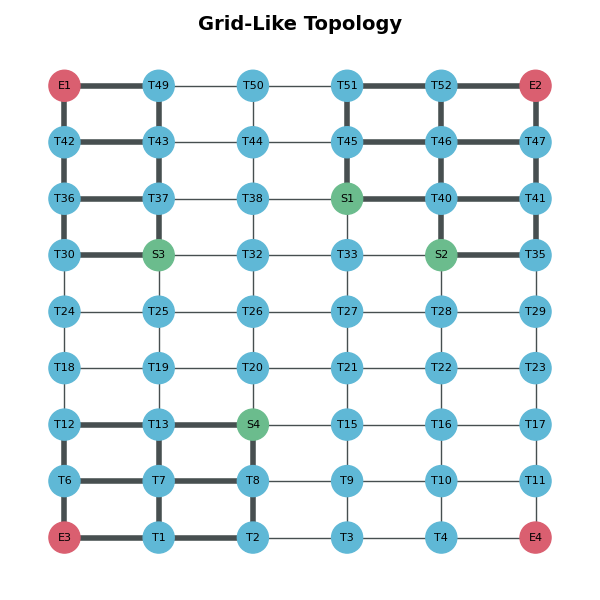
\includegraphics[width=0.3\textwidth]{dissertation_images/grid-like_topology.png}
    \hfill
    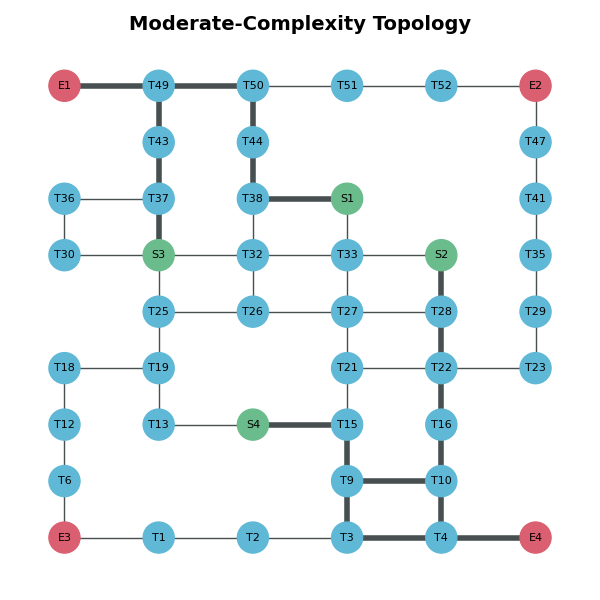
\includegraphics[width=0.3\textwidth]{dissertation_images/moderate-complexity_topology.png}
    \hfill
    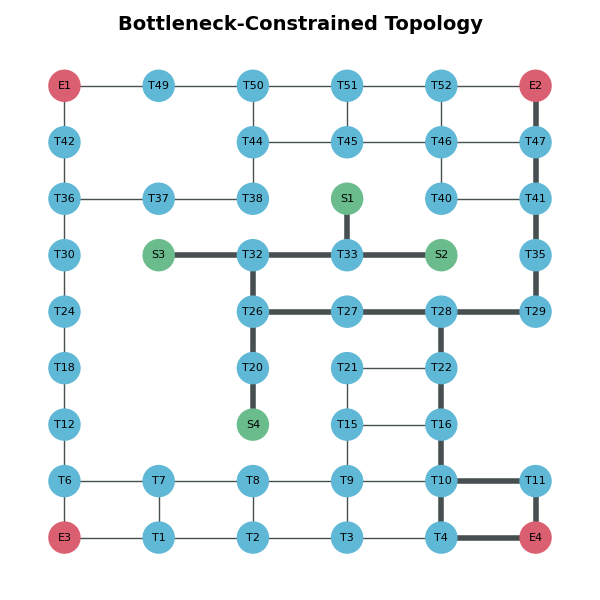
\includegraphics[width=0.3\textwidth]{dissertation_images/bottleneck-constrained_topology.png}
    \caption[Grid, Moderate and Bottleneck Topologies]{Network topologies from left to right; grid-like, moderate-complexity and bottlneck-constrained. The green nodes represent starting positions (S) and red exit positions (E).}
    \label{fig:network-topologies}
\end{figure}

The grid-like topology is the unmodified 6x9 grid and represents a highly connected urban layout with many alternative routes to safety. This topology provides a baseline case in which congestion is less constrained by the network itself. The moderate complexity was created removing ten nodes to create a network which had fewer route options with some exits less accessible and start nodes with overlapping shortest paths. In particular, the overlap between the nearest exits of S1 and S3 creates a useful test of whether the genetic algorithm can redirect agents away from congestion towards underutilised exits. The bottleneck-constrained topology was generated by removing additional nodes and edges to create a limited path choice at the start of the network. It is intended to test how each algorithm behaves when early route choice is heavily restricted and the closest exit is not necessarily the best option for the whole population. 

To validate that these topologies were distinct they were assessed against four metrics: average path length, maximum betweenness, edge density and critical edge load. The results in \autoref{table:topology-metrics} show that the metrics all increase in the expected direction, indicating progressively more constrained routing across the three graphs.

\begin{table}[htb]
  \bigskip
  \begin{center}
    \begin{tabular}{| l | >{\centering\arraybackslash}p{2.5cm} | >{\centering\arraybackslash}p{2.5cm} | >{\centering\arraybackslash}p{2.5cm} | >{\centering\arraybackslash}p{2.5cm} |}
      \hline
      Topology & Mean Path Length & Max Betweeness & Edge Density & Critical Edge Load \\
      \hline
      \hline
      Grid-Like & 6.5 & 0.00122	& 0.0649 & 0.000893\\
      Moderate-Complexity & 7.0 &	0.00249 &	0.0581 & 0.002114\\
      Bottlneck-constrained & 11.5 & 0.00740 & 0.0531 & 0.007092\\
      \hline
    \end{tabular}
  \end{center}
\caption[Topolgoy Metrics]{Metrics for each topology to ensure they were unique.}
\label{table:topology-metrics}
\end{table}

Although the three topologies provide a controlled way to compare routing behaviour under different structural conditions, they remain simplified and idealised representations of real evacuation networks. The results should be interpreted as evidence of relative performance rather than a direct prediction.

\section{Agent Implmentation}
\subsection{Characteristic Assignment}
In order to ensure that the agents had the same characteristics across both the genetic algorithm and greedy the characteristics were generated in advance and passed into the PopulationCreation class for assignment to each of the agents. \autoref{fig:agent-characteristics} show the resulting distributions for the agent characteristics across 100 agents and 10 seeds. The distributions appear stable across the seeds while still shows sampling noise which should balance out in the final results.

\begin{figure}[h]
    \centering
    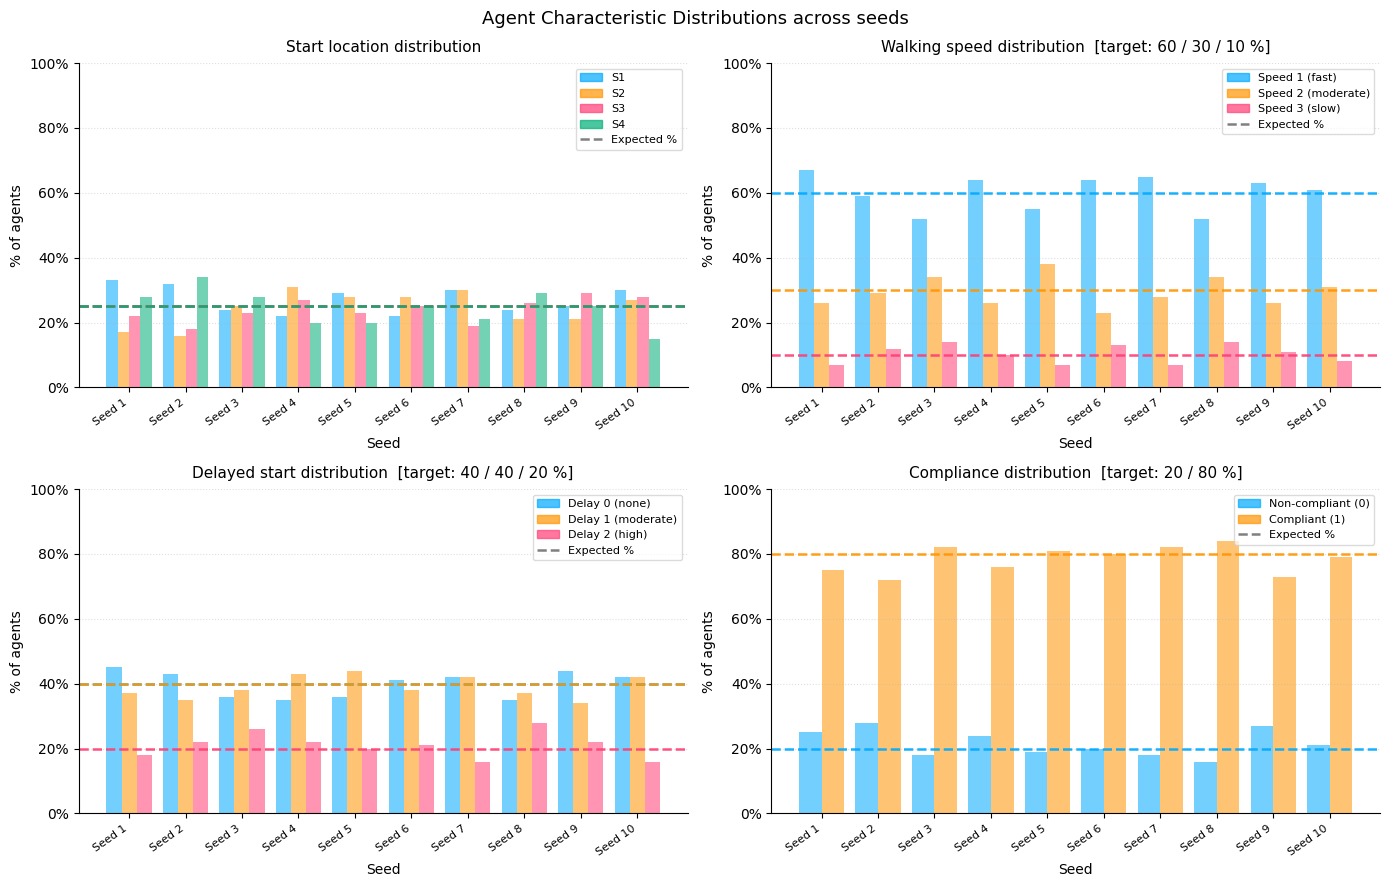
\includegraphics[width=0.9\textwidth]{dissertation_images/agent_characteristics_across_seeds.png}
    \caption[Agent Characteristics across 10 seeds]{Agent Characteristics across 10 seeds for start location (top-left), walking speed (top-right), delayed starts (bottom left) and 80\% compliance rate (bottom-right).}
    \label{fig:agent-characteristics}
\end{figure}


\subsection{Reproducibility Validation}
In order to ensure reproducibility across the algorithms a KeyManager class was utilised and passed into each of the classes which required randomness. Each experiment takes a seed value which is passed to the key manager to split using a JAX PRNG key to produce a reproducible sequence of random keys. In the GA, these keys used to generate probability thresholds in the crossover and mutation operators. Whilst in the greedy algorithm the seed is used to randomly pick the shortest path.

An early implementation passed the seeds directly through the algorithm, however upon investigation found that the seed was being repeated producing the same crossover probabilities each time. This was resolved by the centralised KeyManager Class. It is worth noting that the results are only reproducible if the same sequence of operators is used as the request to the key manager must be consistent across the runs. 

\section{Greedy Algorithm Implementation}
For the greedy shortest path implementation, NetworkX’s shortest path function was used, however it was found that the default behaviour returns the first shortest path encounter (breadth first search) which causes all agents starting from the same node to follow the same route. This created artificial congestion levels from the path selection rather than the network structure itself. To avoid this, the implementation was modified to find all shortest paths and if there is more than one, then one is selected at random. This ensures all agents are split across equivalent routes in a way which better reflects real evacuations. \autoref{fig:greedy-routing-options} shows across three different seeds randomly selecting the shortest path versus the selecting the first path. This ensures the greedy algorithm is a fairer baseline comparison against the GA, as if first-found paths were used, the greedy approach would unfairly overstate congestion.

\begin{figure}[h]
    \centering
    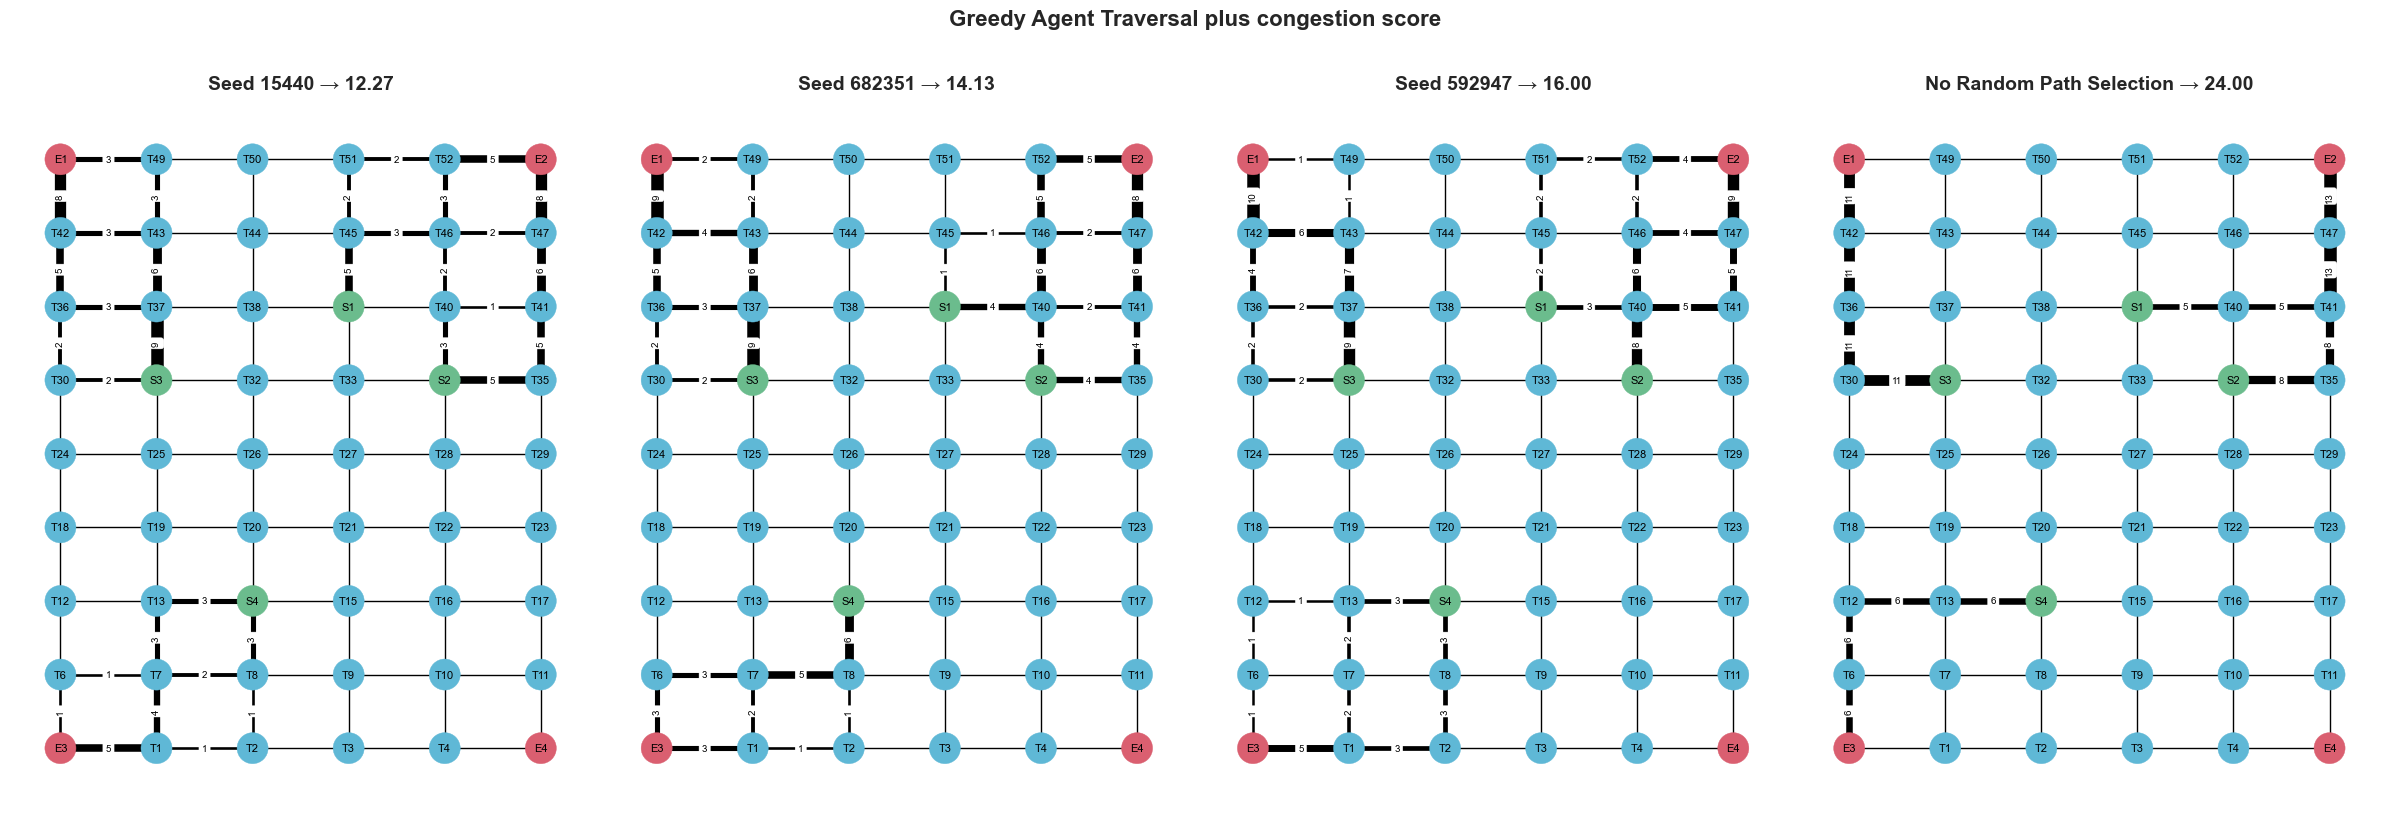
\includegraphics[width=1\textwidth]{dissertation_images/greedy_shortest_path_random_or_first.png}
    \caption[Greedy Shortest Path Routing Options]{Greedy shortest path routing options across 3 seeds (from left) and first path selection (right). The thicker the edge weight in the figure show the frequency of use which varies across the seeds}
    \label{fig:greedy-routing-options}
\end{figure}

\section{Genetic Algorithm Tuning}
A sequential tuning approach was taken to tune the parameters due to the high computational cost of a full grid search. All the parameters were tested across multiple seeds on the moderate-constrained topology. The potential options can be found in \autoref{table:ga-parameters} and final selection at the end of this section.

\subsection{Initial Parameter Tuning}
The mean and standard deviation of the metrics in \autoref{table:experiment-metrics} was used to assess hyperparameter performance, with total time being the primary decision metric.

The epsilon parameter which produced the best results was $\epsilon=1$. This is notable because the original purpose of this parameter was to preserve some randomness in the rerouting process; however, at this value the mutation step almost becomes fully greedy. This is less concerning than it first appears, because the greedy path is made to a randomly selected exit, rather than always to the nearest one, so some variation in route choice is still retained at exit selection.

For the mutation rate, a wider range of values was selected for the mutation rate as the mutation appears on the agent level not at the chromosome level and a higher level of exploration across the routes was desired. The best choice based purely on total time would have been 0.01, however in order to ensure that exploration is happening the 0.05 mutation rate was selected initially instead.

For the population size parameter, the chosen value was 50, although both population sizes 100 and 200 did improve the total time and average path length, they did not improve the performance enough to warrant the increase in computational costs and time required to run the larger populations.

\subsection{Operator Selection Methods}
Next the parent and survivor selection operators were tuned together. For the survivor selection elite percentage, either 10 parents or 10\% of the population size were kept, whichever was bigger and the remaining filled with children. Again the metrics from \autoref{table:experiment-metrics} were used alongside \autoref{table:parent-selection}. \autoref{fig:parent-selection-small-mutation} shows the results of those metrics across 20 seeds for mutation probability 0.05.

\begin{figure}[h]
    \centering
    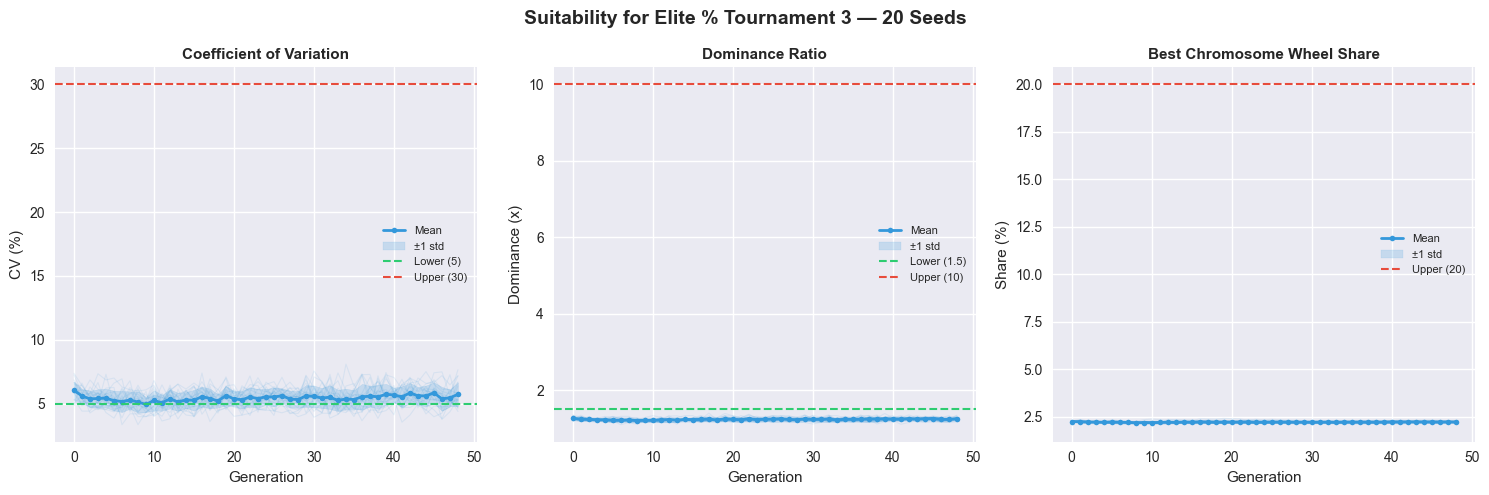
\includegraphics[width=0.9\textwidth]{dissertation_images/selection_methods_tournament_elite_percentage.png}
    \caption[Tournament (N=3) and Elite Percentage Performance]{Tournament (N=3) and Elite Percentage Performance across 20 seeds for (left) cofficient of variance, dominance ratio and best wheel share, with 0.05 mutation probability.}
    \label{fig:parent-selection-small-mutation}
\end{figure}

In addition to the parent selection metrics, the performance of the fitness function across the generations for each survivor selection method was analysed, \autoref{fig:survivor-selection-plot}. Additional selection method plots can be found in \autoref{chap:results}

\begin{figure}[h]
    \centering
    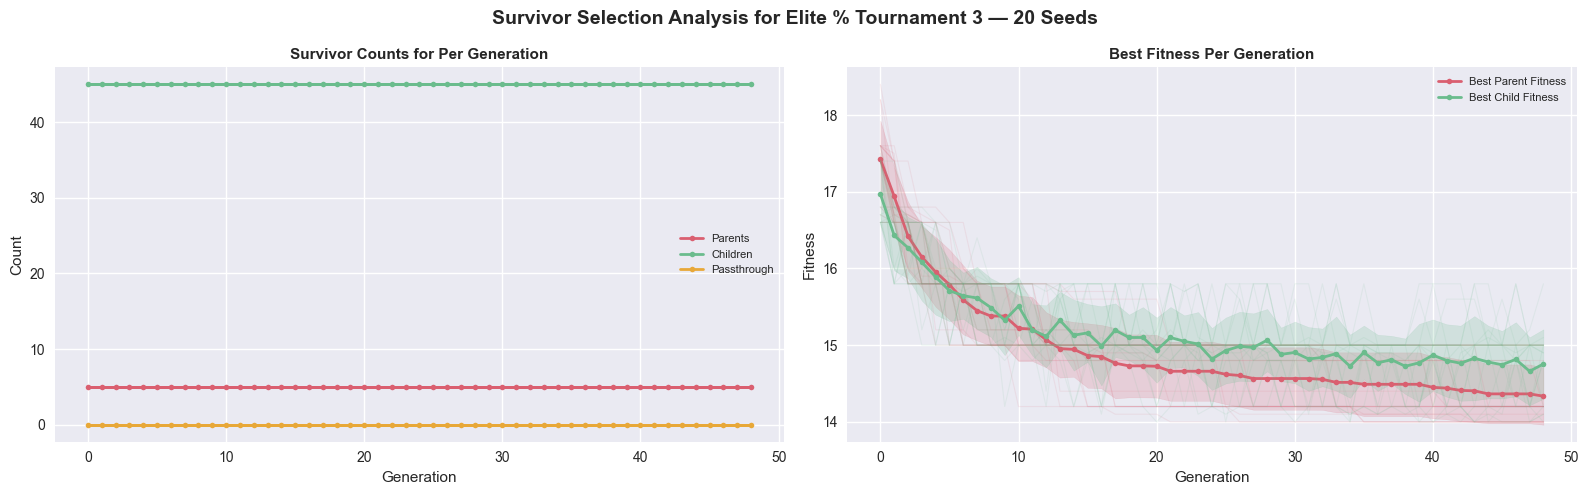
\includegraphics[width=0.9\textwidth]{dissertation_images/survivor_elite_perc_tournament_3.png}
    \caption[Survivor Selection Fitness Functions]{Elite percentage survivor selection results across 20 seeds, (left) shows the proportion of child, parent and passthrough chromosomes at the end of each evolution and (right) shows the best fitness per generation across the parent and child chromosomes.}
    \label{fig:survivor-selection-plot}
\end{figure}

The purely elite vs an elite percentage had similar results but the elite percentage with tournament selection of size 3 had the best total and average time across the seeds and appeared to have better diversity through the evolutions so was selected as the parameter going forward. It is worth noting that for almost all the combinations run at mutation rate 0.05 the coefficient of variance results lay very close to the 5\% boundary set previously and the dominance ratio below the x1.5 boundary. As a result, some of the experiments were run again with the mutation probability increased to 0.1, \autoref{fig:parent-selection-bigger-mutation}, these showed more promising results, so the mutation probability was increased to this.


\begin{figure}[h]
    \centering
    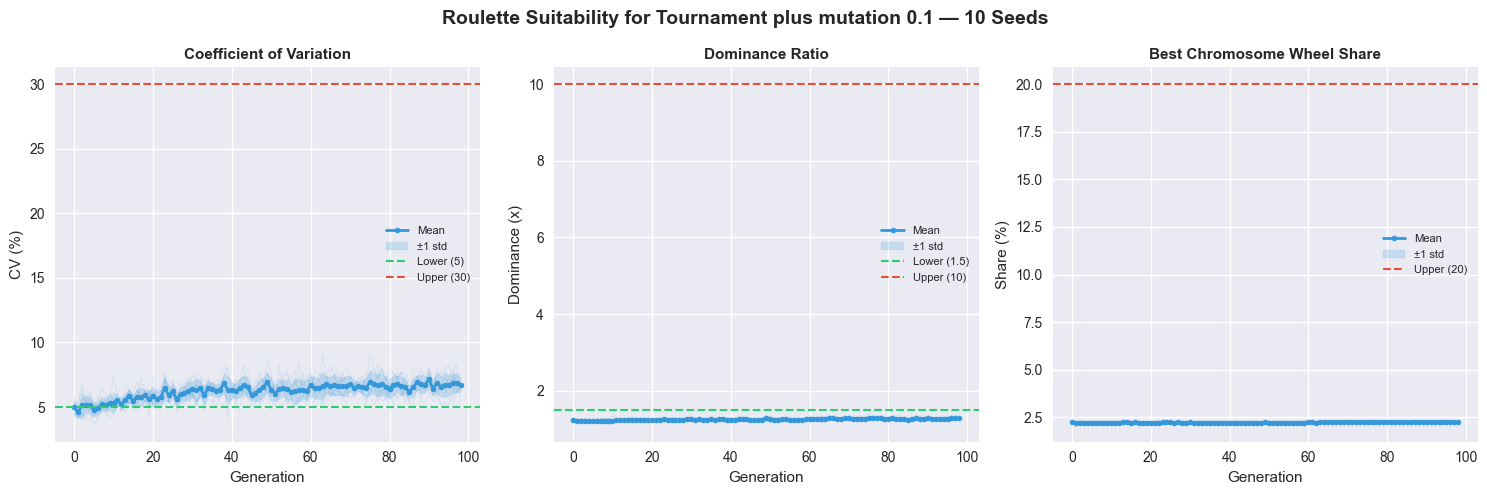
\includegraphics[width=0.9\textwidth]{dissertation_images/tournament_mutation_1.png}
    \caption[Parent and Survivor Selection with modified mutation]{Tournament (N=3) and Elite Percentage Performance across 20 seeds for (left) cofficient of variance, dominance ratio and best wheel share, with 0.1 mutation probability.}
    \label{fig:parent-selection-bigger-mutation}
\end{figure}

\subsection{Agent Tuning}
The number of agents used in the simulation was tuning in order to ensure the right amount of congestion was observed, as a result this was done across all topologies, comparing across both algorithms (\autoref{fig:num-agents-ga}, \autoref{fig:num-agents-greedy}).

\begin{figure}[h]
    \centering
    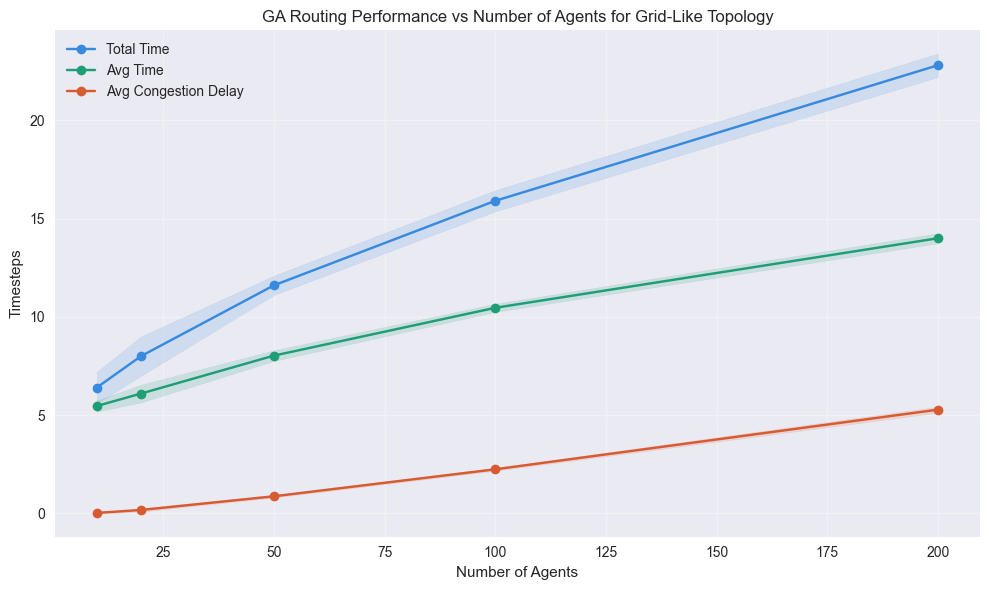
\includegraphics[width=0.3\textwidth]{dissertation_images/grid_topology_ga_num_agents.png}
    \hfill
    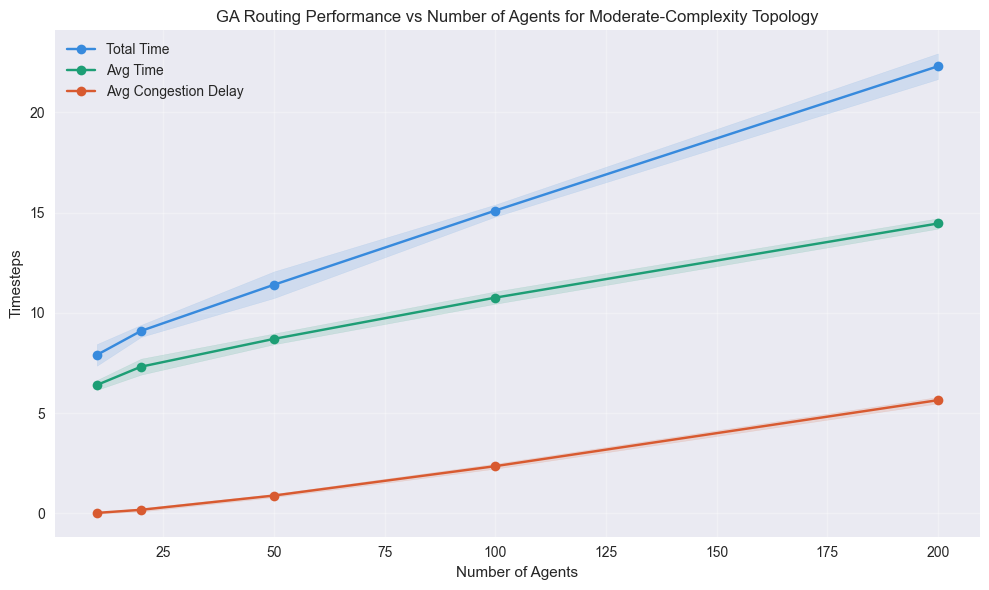
\includegraphics[width=0.3\textwidth]{dissertation_images/moderate_topology_ga_num_agents.png}
    \hfill
    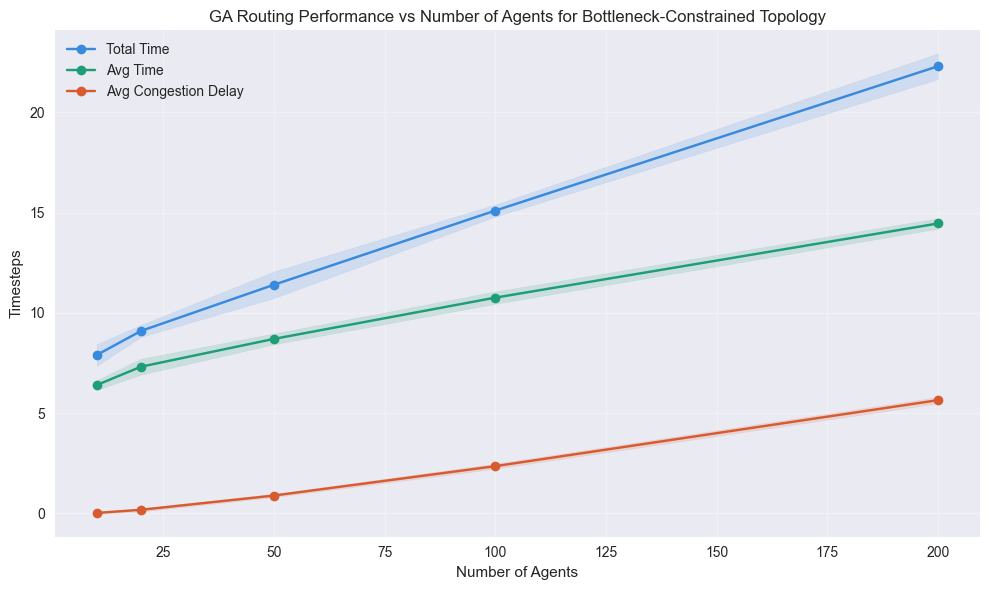
\includegraphics[width=0.3\textwidth]{dissertation_images/bottlneck_topology_ga_num_agents.png}
    \caption[Analysis number of agents for genetic algorithm]{From left to right, Grid, Moderate and Bottleneck Topologies number of agents vs Fitness Function for genetic algorithm.}
    \label{fig:num-agents-ga}
\end{figure}

\begin{figure}[h]
    \centering
    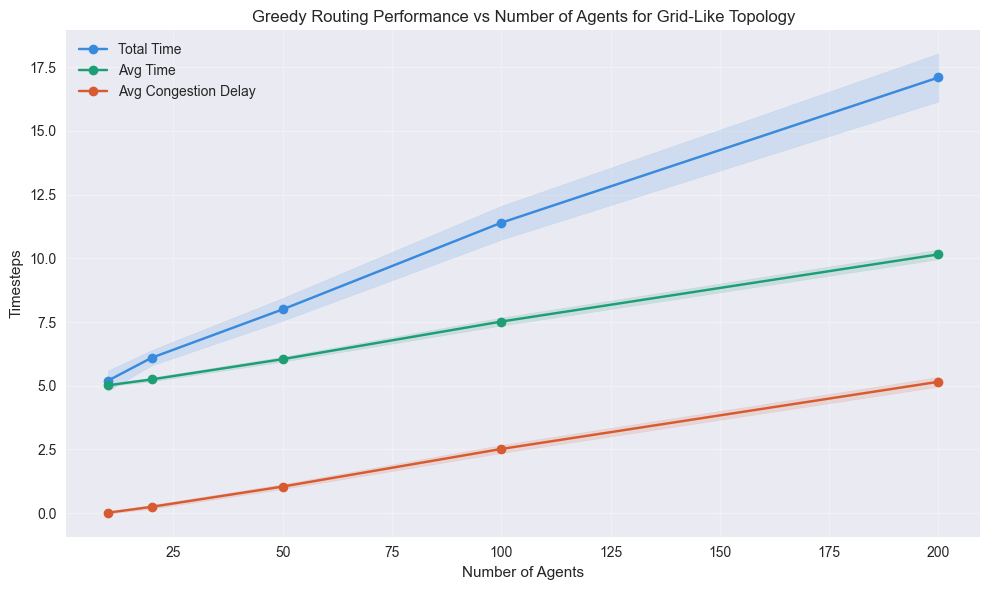
\includegraphics[width=0.3\textwidth]{dissertation_images/grid_topology_greedy_num_agents.png}
    \hfill
    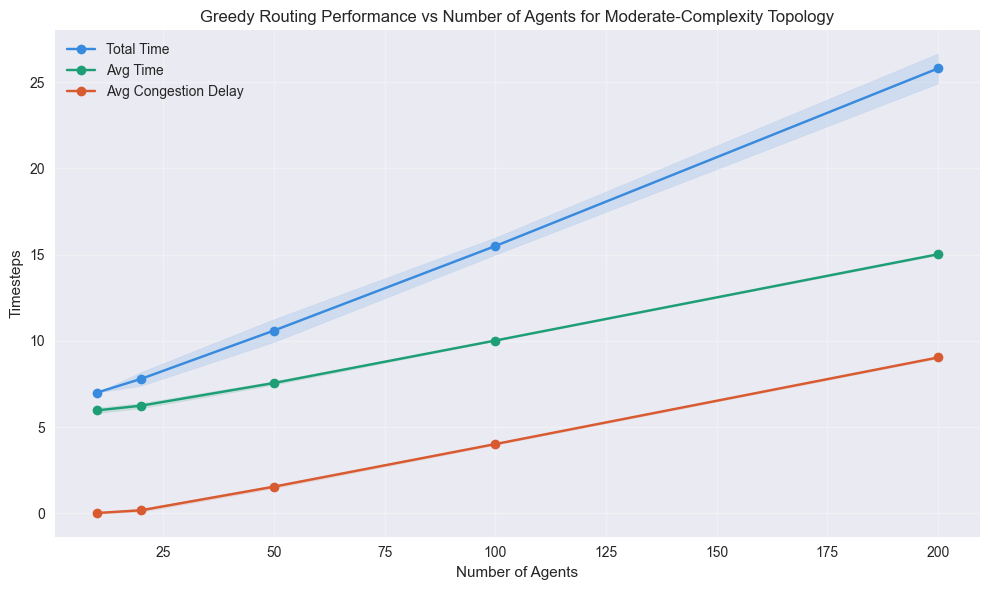
\includegraphics[width=0.3\textwidth]{dissertation_images/moderate_topology_greedy_num_agents.png}
    \hfill
    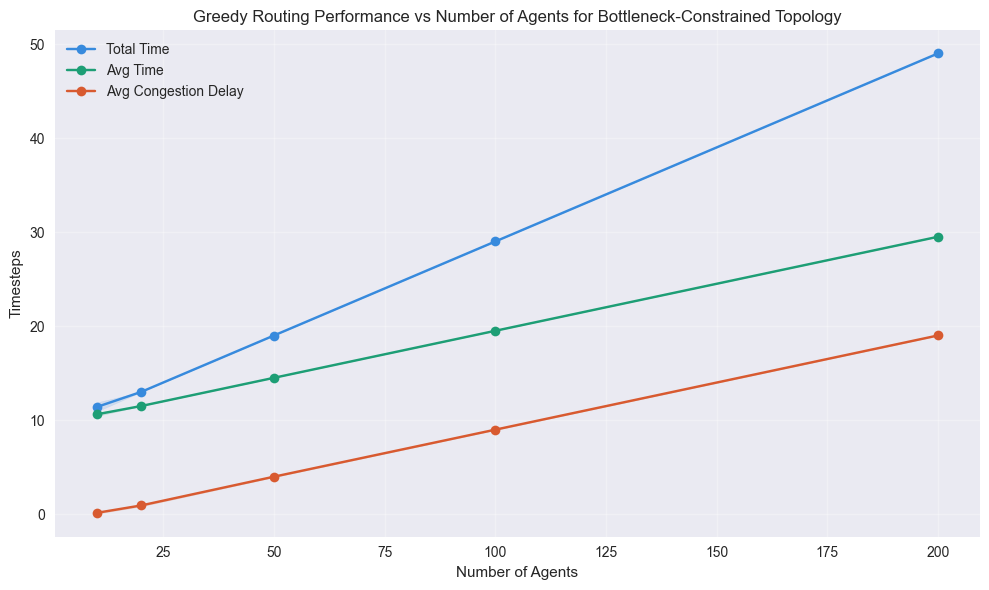
\includegraphics[width=0.3\textwidth]{dissertation_images/bottlneck_topology_greedy_num_agents.png}
    \caption[Analysis number of agents for greeedy algorithm]{From left to right, Grid, Moderate and Bottleneck Topologies number of agents vs Fitness Function for greedy algorithm.}
    \label{fig:num-agents-greedy}
\end{figure}

The number of agents selected for the main experiments is 100. This provides enough congestion to demonstrate the benefit of global optimisation, while avoiding the risk of overload seem in the 200-agent case and could result in the simulation being dominated by congestion. Using 100 agents across all topologies also keeps the comparison consistent between scenarios meaning different population sizes don’t need to be picked per topology. This simplifies the experimental design, although using fewer agents for the bottleneck topology could reduce the computation required.

\subsection{Maximum Evolutions}
The termination criteria (max evolutions) was the last parameter tuned for all topologies to ensure convergence. \autoref{fig:max-evolutions} shows the best, mean and worst fitness scores for 200 evolutions across 10 seeds. Based on these results, a maximum of 100 generations was set, as the fitness function had generally plateaued by around 50 generations across all topologies. The additional 50 generations were retrained as a buffer to allow slower converging runs to stabilise, which is especially important for the bottleneck topology.

\begin{figure}[h]
    \centering
    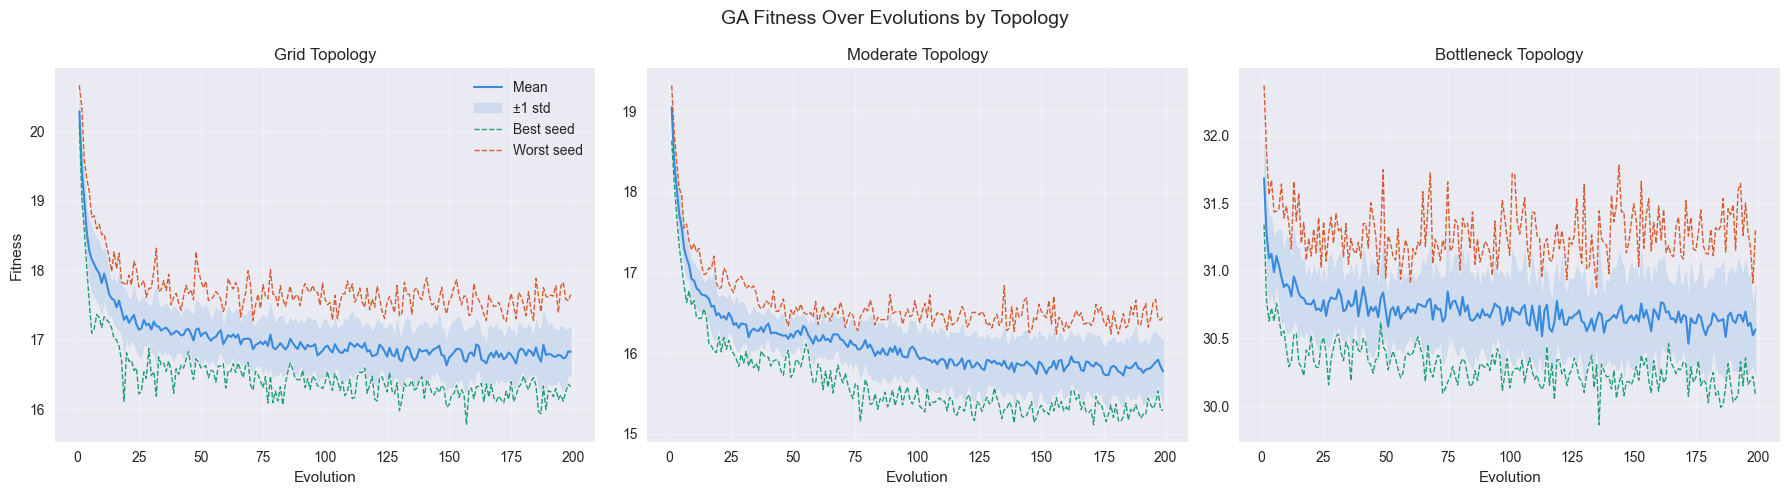
\includegraphics[width=0.9\textwidth]{dissertation_images/GA_fitness_over_topology.png}
    \caption[Genetic Algorithm fitness over evolutions]{Genetic Algorithm best (green), mean (blue) and worst (red) fitness over evolutions across 10 seeds to decide termination criteria.}
    \label{fig:max-evolutions}
\end{figure}

However, the worst seed value (red) does raise some concern as it does not appear to fully converge even after 200 generations. This suggests the sequential tuning process may not have captured seed level variations in the convergence behaviour, since the metrics were aggregated to the final generation rather than the full evolutionary trajectory.

\section{Summary of Implementation Decisions}
Overall, the implementation was designed to produce a reproducible and controlled framework for comparing the greedy baseline and genetic algorithm under identical conditions. The main developments focused on developing these algorithms, environments and agent characteristics then fixing the parameters before the main experiments, \autoref{table:ga-final-params}.

\begin{table}[htb]
  \bigskip
  \begin{center}
    \begin{tabular}{|l|l|}
      \hline
      Parameter & Value \\
      \hline
      \hline
      Fitness Aggregation & $(\alpha * \max - (1-\alpha)*median)$ $\alpha = 0.8$ \\
      Epsilon & 1 \\
      Crossover Probability & 0.8 \\
      Mutation Probability & 0.1 \\
      Population Size & 50 \\
      Parent Selection Method & Tournament Selection (N=3) \\
      Survivor Selection Method & Elite Percentage \\
      Number of Agents & 100 \\
      Maximum Evolutions & 100 \\
      \hline
    \end{tabular}
  \end{center}
\caption[Final parameters for the Genetic Algorithm]{Final parameters selected the for Genetic Algorithm from sequential tuning.}
\label{table:ga-final-params}
\end{table}



%%%%%%%%%%%%%%%%%%%%%%%%%%%%%%%%%%%%%%%%%%%%%%%%%%%%%%%%%%%%%%%%%%%%%%%%%%%%%%%%

\chapter{Useful stuff}

\section[Short Section Title]{Another Section With a Long Title and Whose Title Is Abbreviated in the Table of Contents}


\begin{figure}[h]
    \centering
    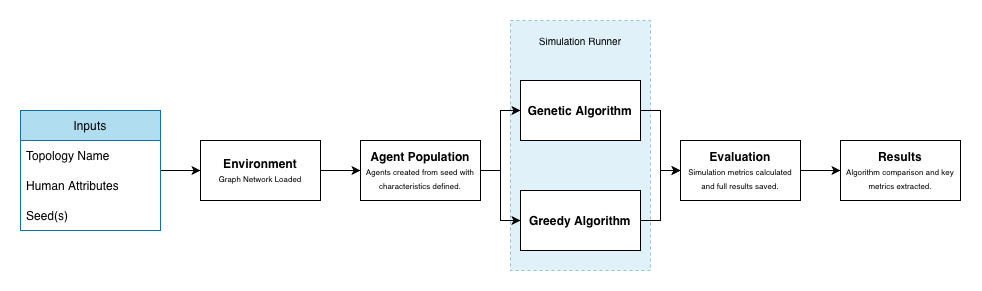
\includegraphics[width=0.8\textwidth]{dissertation_images/architecture_diagram_design.png}
    \caption[Architecture Diagram]{Architecture diagram showing the  project framework connecting the input parameters through environment, agent creation, routing algorithms and evaluation.}
    \label{fig:architecture-design}
\end{figure}

%-------------------------------------------------------------------------------
\begin{table}[htb]
  \bigskip
  \begin{center}
    \begin{tabular}{|l|l|}
      \hline
      Items & Values \\
      \hline
      \hline
      Item 1 & Value 1 \\
      Item 2 & Value 2 \\
      \hline
    \end{tabular}
  \end{center}
\caption{An example table}
\label{Example-Table}
\end{table}

Another section, just for good measure. You can reference a table, figure or equation using \verb|\ref|, just like this reference to Table \ref{Example-Table}.

\section{Example Lists}

%-------------------------------------------------------------------------------
\subsection{Enumerated}

\begin{enumerate}
\item Example enumerated list:
  \begin{itemize}
  \item a nested enumerated list item;
  \item and another one.
  \end{itemize}
\item Second item in the list.
\end{enumerate}

%-------------------------------------------------------------------------------
\subsection{Itemised}

\begin{itemize}
\item Example itemised list.
  \begin{itemize}
  \item A nested itemised list item.
  \end{itemize}
\item Second item in the list.
\end{itemize}

%-------------------------------------------------------------------------------
\subsection{Description}

\begin{description}
\item[Item 1]First item in the list.
\item[Item 2]Second item in the list.
\end{description}

%%%%%%%%%%%%%%%%%%%%%%%%%%%%%%%%%%%%%%%%%%%%%%%%%%%%%%%%%%%%%%%%%%%%%%%%%%%%%%%%

%%%%%%%%%%%%%%%%%%%%%%%%%%%%%%%%%%%%%%%%%%%%%%%%%%%%%%%%%%%%%%%%%%%%%%%%%%%%%%%%
\chapter{Results}

This is the chapter in which you present the results. You may include user evaluation here too.

%%%%%%%%%%%%%%%%%%%%%%%%%%%%%%%%%%%%%%%%%%%%%%%%%%%%%%%%%%%%%%%%%%%%%%%%%%%%%%%%
%%%%%%%%%%%%%%%%%%%%%%%%%%%%%%%%%%%%%%%%%%%%%%%%%%%%%%%%%%%%%%%%%%%%%%%%%%%%%%%%
\chapter{Discussion}

This is the chapter in which you clearly review the results, and critique the process. You must end this chapter with a discussion of the implication of the results, acknowledging the limitations of your work, and identifying possible future work.  

%%%%%%%%%%%%%%%%%%%%%%%%%%%%%%%%%%%%%%%%%%%%%%%%%%%%%%%%%%%%%%%%%%%%%%%%%%%%%%%%
%%%%%%%%%%%%%%%%%%%%%%%%%%%%%%%%%%%%%%%%%%%%%%%%%%%%%%%%%%%%%%%%%%%%%%%%%%%%%%%%
\chapter{Conclusions}

%%
%% Now we are back to the standard project contents that you should include
%%

This is the chapter in which you summarise the entire project, review the major achievements in the light of your original objectives.

\vfill
Number of words until this point, excluding front matter: XXX.

%%%%%%%%%%%%%%%%%%%%%%%%%%%%%%%%%%%%%%%%%%%%%%%%%%%%%%%%%%%%%%%%%%%%%%%%%%%%%%%%
%%%%%%%%%%%%%%%%%%%%%%%%%%%%%%%%%%%%%%%%%%%%%%%%%%%%%%%%%%%%%%%%%%%%%%%%%%%%%%%%
\bibliography{EndNotesTest}

%%%%%%%%%%%%%%%%%%%%%%%%%%%%%%%%%%%%%%%%%%%%%%%%%%%%%%%%%%%%%%%%%%%%%%%%%%%%%%%%
%%%%%%%%%%%%%%%%%%%%%%%%%%%%%%%%%%%%%%%%%%%%%%%%%%%%%%%%%%%%%%%%%%%%%%%%%%%%%%%%
\appendix

%%
%% Use the appendix for major chunks of detailed work, such as these. Tailor
%% these to your own requirements
%%

%%%%%%%%%%%%%%%%%%%%%%%%%%%%%%%%%%%%%%%%%%%%%%%%%%%%%%%%%%%%%%%%%%%%%%%%%%%%%%%%
%%%%%%%%%%%%%%%%%%%%%%%%%%%%%%%%%%%%%%%%%%%%%%%%%%%%%%%%%%%%%%%%%%%%%%%%%%%%%%%%
\chapter{Design Diagrams}

% latex_dissertation/dissertation_images/appendix_diagrams/genetic_algortihm_process.png

\chapter{Results Diagrams}
\label{chap:results}

The following plots show the different performance of the parent selection and survivor selection tuning:

% appendix_diagrams/parent_selection_performance_metrics_plots.png



% \begin{figure}[h]
%     \centering
%     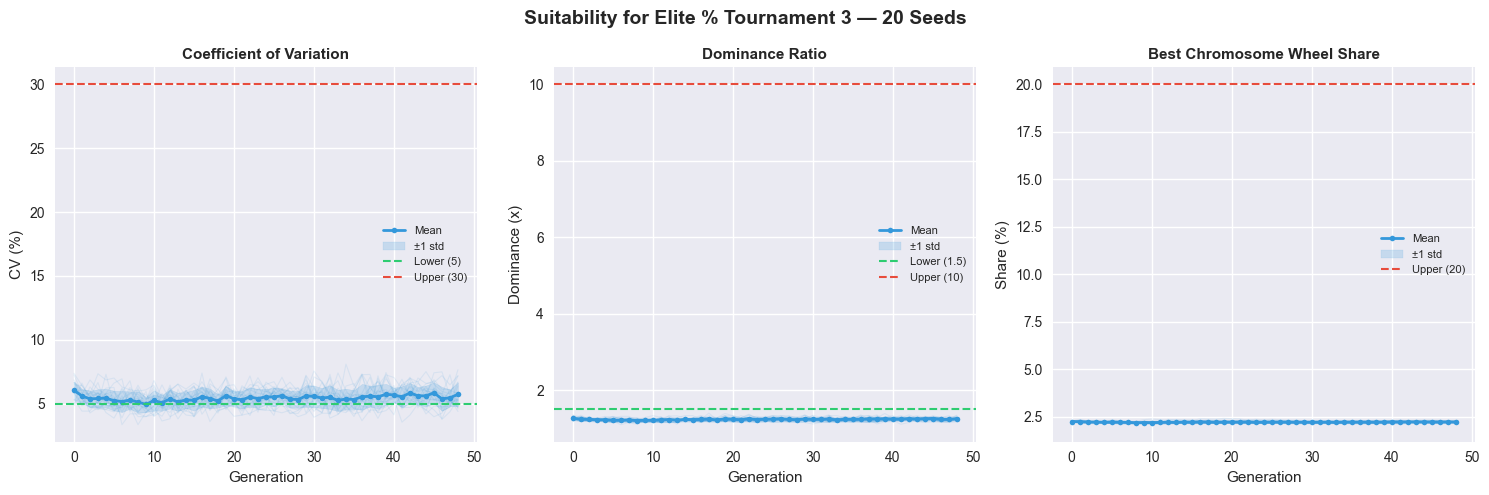
\includegraphics[width=0.9\textwidth]{dissertation_images/selection_methods_tournament_elite_percentage.png}
%     \caption{TODO}
%     \label{fig:parent-selection-small-mutation}
% \end{figure}

% \begin{figure}[h]
%     \centering
%     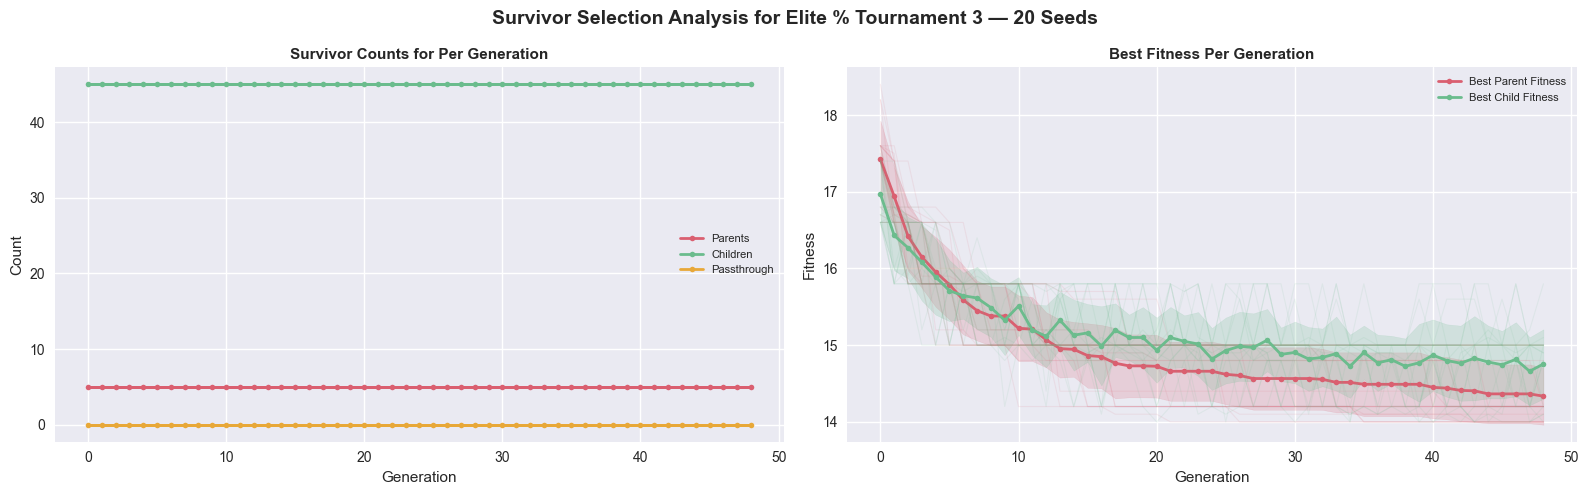
\includegraphics[width=0.9\textwidth]{dissertation_images/survivor_elite_perc_tournament_3.png}
%     \caption[Survivor Selection Fitness Functions]{Elite percentage survivor selection results across 20 seeds, (left) shows the proportion of child, parent and passthrough chromosomes at the end of each evolution and (right) shows the best fitness per generation across the parent and child chromosomes.}
%     \label{fig:survivor-selection-plot}
% \end{figure}


%%%%%%%%%%%%%%%%%%%%%%%%%%%%%%%%%%%%%%%%%%%%%%%%%%%%%%%%%%%%%%%%%%%%%%%%%%%%%%%%
%%%%%%%%%%%%%%%%%%%%%%%%%%%%%%%%%%%%%%%%%%%%%%%%%%%%%%%%%%%%%%%%%%%%%%%%%%%%%%%%
\chapter{User Documentation}

% CODE BASE LINK

%%%%%%%%%%%%%%%%%%%%%%%%%%%%%%%%%%%%%%%%%%%%%%%%%%%%%%%%%%%%%%%%%%%%%%%%%%%%%%%%
%%%%%%%%%%%%%%%%%%%%%%%%%%%%%%%%%%%%%%%%%%%%%%%%%%%%%%%%%%%%%%%%%%%%%%%%%%%%%%%%
\chapter{Raw Results Output}

%%%%%%%%%%%%%%%%%%%%%%%%%%%%%%%%%%%%%%%%%%%%%%%%%%%%%%%%%%%%%%%%%%%%%%%%%%%%%%%%
%%%%%%%%%%%%%%%%%%%%%%%%%%%%%%%%%%%%%%%%%%%%%%%%%%%%%%%%%%%%%%%%%%%%%%%%%%%%%%%%
\chapter{Code}

%% NOTE For this to typeset correctly, ensure you use the pdflatex
%%      command in preference to the latex command.  If you do not have
%%      the pdflatex command, you will need to remove the landscape and
%%      multicols tags and just make do with single column listing output

\begin{landscape}
\begin{multicols}{2}
\section{File: yourCodeFile.java}
\lstinputlisting[basicstyle=\scriptsize]{yourCodeFile.java}
\end{multicols}
\end{landscape}

\end{document}
